\documentclass[a4paper,12pt]{article}
\usepackage[utf8]{inputenc}  
\usepackage{geometry}        
\usepackage{graphicx}
\usepackage{xcolor}
\usepackage{listings}
\usepackage{todonotes}
\usepackage{multicol}
\usepackage{float}
\geometry{a4paper, margin=2cm}

\definecolor{darkred}{rgb}{0.6, 0.0, 0.0}   
\definecolor{darkgreen}{rgb}{0.0, 0.5, 0.0}  
\definecolor{darkblue}{rgb}{0.0, 0.0, 0.6} 
\definecolor{darkyellow}{rgb}{0.8, 0.7, 0.0}

\newcommand{\myparagraph}[1]{\paragraph{#1}\mbox{}\\}

\title{Documentation for ITW project}
\author{Jerry Huang}
\date{2023-2024}


\begin{document}
\maketitle
\begin{center}
\includegraphics[width=0.5\textwidth]{Logo.png}
\end{center}
\newpage
\tableofcontents
\listoffigures

\newpage


\section{Introduction}

The project involves the creation of a web application dedicated to document management, developed using technologies such as Java, HTML, and CSS. The website will be available in two variants for client-side scripting: one based on Thymeleaf and the other on JavaScript.\\ Each version will provide users with specific functionalities based on the technology used. Users will have access to various options for managing, viewing, and organizing documents.\\ The application provides user login and registration functionality via a public page. It then checks the email and password, ensuring the syntactic validity of both and the uniqueness of the username. Each folder is characterized by a name, creation date, and can contain other folders or documents. Documents include information such as owner, name, creation date, summary, and document type. 

\subsection{Pure HTML}
After the user logs in, a homepage appears displaying a tree of their folders and subfolders.
\begin{figure}[h]
    \centering
    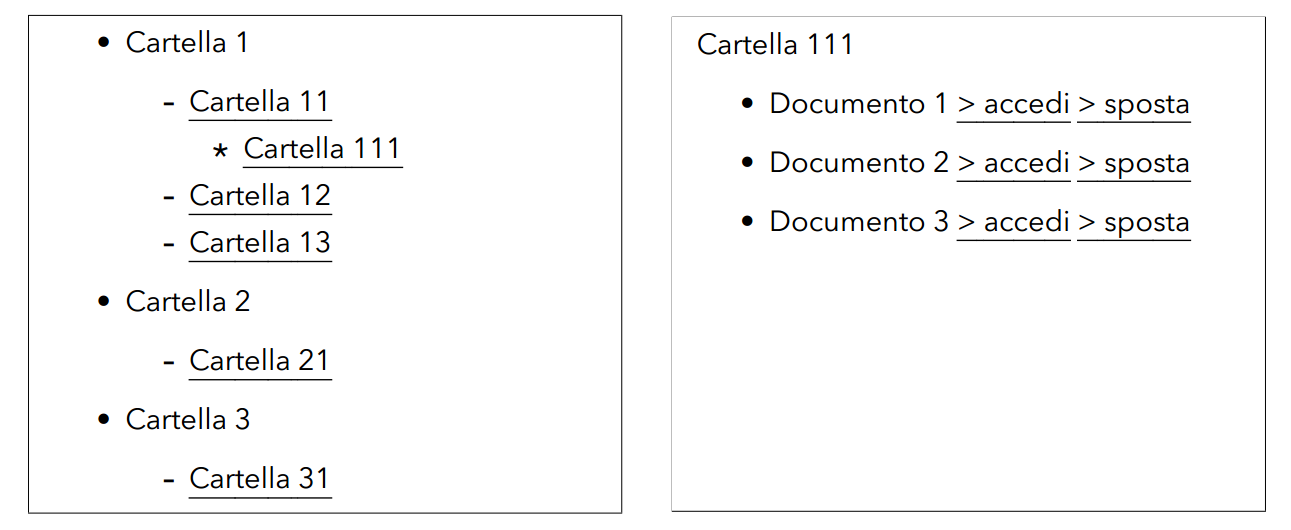
\includegraphics[width=1.0\textwidth]{HTML/HTMLTree.png}
    \caption{Image from the teacher's project requirements.}
    \label{fig:HTMLTree}
\end{figure}
On the homepage, the user can select a folder and access a contents page, which shows a list of folders and documents within the selected folder. Each document has two links: "access" and "move". If the user clicks on "access", the document page appears showing the details of the selected document. If "move" is clicked, the homepage reappears with a message saying "You are moving document X from folder Y. Choose a destination folder." The folder containing the document is not selectable, and its name is highlighted. Once the user selects the destination folder, the document is moved, and the contents page of the destination folder is displayed. Every page, except the homepage, contains a link to return to the previous page. The user can log out from any page. Finally, a content management page, accessible from the homepage, allows the user to create a top-level folder, a subfolder inside an existing folder, or a document inside a folder.

\newpage
\subsection{JavaScript}
The application still supports login and registration, and in addition to the syntax validation of the email, the equality of the "password" and "repeat password" fields is also checked on the client and server side. After the user logs in, the entire application is implemented on a single page. Error messages are displayed within the page for the user to see. The movement of documents or folders occurs via drag and drop. Next to each folder, two labeled buttons appear "add subfolder" and "add document", they respectively trigger a form to input the name of the subfolder or the document details. Finally, a folder called "trash bin" is added; dragging a document into the trash results in its deletion. Before deleting the document, a confirmation window appears. Deleting a folder results in the complete and recursive deletion of all data (documents and subfolders).
\subsection{Additional notes}
\begin{itemize}
	\item{Since the project involves developing two versions of the same	application with only minor modifications, the database remains unchanged as it needs to be accessed by both versions.}
	\item{Upon registration, each user is assigned a root folder. All subsequent folders and documents must be created within this root folder. This approach simplifies the database by maintaining a clear, linear tree structure, similar to the organization of a traditional file system on a PC.}
\end{itemize}
\newpage

\section{Database design}
\subsection{Database design}
\paragraph{Data requirements}
[\textcolor{darkred}{Entities} \textcolor{darkgreen}{Attributes} \textcolor{darkblue}{Relationships}]\\
The application provides \textcolor{darkred}{user} login and registration functionality via a public page. It then checks the \textcolor{darkgreen}{email} and \textcolor{darkgreen}{password}, ensuring the syntactic validity of both and the uniqueness of the \textcolor{darkgreen}{username}. Each \textcolor{darkred}{folder} is characterized by a \textcolor{darkgreen}{name}, \textcolor{darkgreen}{creation date}, and \textcolor{darkblue}{ contain other folders or documents}. \textcolor{darkred}{Documents} include information such as \textcolor{darkgreen}{owner}, \textcolor{darkgreen}{name}, \textcolor{darkgreen}{creation date}, \textcolor{darkgreen}{summary}, and \textcolor{darkgreen}{document type}.

\myparagraph{SQL Code}
\lstset{
  language=SQL,
  basicstyle=\ttfamily\footnotesize,
  keywordstyle=\color{blue},
  breaklines=true,      
  breakatwhitespace=true 
}
\begin{lstlisting}
CREATE TABLE `document` (
  `DocumentId` int unsigned NOT NULL AUTO_INCREMENT,
  `Owner` int unsigned NOT NULL,
  `Name` varchar(45) NOT NULL,
  `Date` date NOT NULL,
  `Type` varchar(45) NOT NULL,
  `FolderLocation` int unsigned NOT NULL,
  `Summary` varchar(255) NOT NULL,
  PRIMARY KEY (`DocumentId`),
  KEY `FK1_idx` (`FolderLocation`),
  KEY `FK2_idx` (`Owner`),
  CONSTRAINT `FK1` FOREIGN KEY (`FolderLocation`) REFERENCES `folder` (`FolderId`) ON DELETE CASCADE ON UPDATE CASCADE,
  CONSTRAINT `FK2` FOREIGN KEY (`Owner`) REFERENCES `user` (`UserId`) ON DELETE CASCADE ON UPDATE CASCADE
) ENGINE=InnoDB AUTO_INCREMENT=73 DEFAULT CHARSET=utf8mb4 COLLATE=utf8mb4_0900_ai_ci

CREATE TABLE `folder` (
  `FolderId` int unsigned NOT NULL AUTO_INCREMENT,
  `Owner` int unsigned NOT NULL,
  `Name` varchar(45) NOT NULL,
  `Date` date NOT NULL,
  `ParentFolder` int unsigned DEFAULT NULL,
  PRIMARY KEY (`FolderId`),
  UNIQUE KEY `Unique_keys` (`Owner`,`Name`,`ParentFolder`),
  KEY `FK3_idx` (`Owner`),
  KEY `FK4_idx` (`ParentFolder`),
  CONSTRAINT `FK3` FOREIGN KEY (`Owner`) REFERENCES `user` (`UserId`) ON DELETE CASCADE ON UPDATE CASCADE,
  CONSTRAINT `FK4` FOREIGN KEY (`ParentFolder`) REFERENCES `folder` (`FolderId`) ON DELETE CASCADE ON UPDATE CASCADE
) ENGINE=InnoDB AUTO_INCREMENT=199 DEFAULT CHARSET=utf8mb4 COLLATE=utf8mb4_0900_ai_ci
  
  CREATE TABLE `user` (
  `UserId` int unsigned NOT NULL AUTO_INCREMENT,
  `Username` varchar(45) NOT NULL,
  `Password` varchar(60) NOT NULL,
  `Email` varchar(45) NOT NULL,
  PRIMARY KEY (`UserId`),
  UNIQUE KEY `Username_UNIQUE` (`Username`)
) ENGINE=InnoDB AUTO_INCREMENT=49 DEFAULT CHARSET=utf8mb4 COLLATE=utf8mb4_0900_ai_ci
\end{lstlisting}
\newpage

\paragraph{Table schema}
\begin{verbatim}
Document(
	DocumentId, //Unique Id of the document
	Owner, //Id of the user who owns the document
	Name, //Name of the document
	Date, //Date of creation
	Type, //Type of document
	FolderLocation //Id of the folder containing the document
)

Folder(
	FolderId, //Unique Id of the folder
	Owner, //Id of the user who owns the folder
	Name, //Name of the folder
	Date, //Date of creation
	ParentFolder //Id of the parent folder containing the folder
)

User(
	UserId, //Unique Id of the user
	Username, //Unique username of the user
	Password, //Hashed text of the password
	Email //Email of the user
)
\end{verbatim}

\newpage
\subsection{Database diagrams}
\begin{figure}[h]
    \centering
    \includegraphics[width=0.8\textwidth]{ERDiagram.png}
    \caption{ER diagram.}
    \label{fig:ERDiagram}
\end{figure}
    
\begin{figure}[h]
    \centering
    \includegraphics[width=1.0\textwidth]{LogicalSchema.png}
    \caption{Logical schema.}
    \label{fig:LogicalSchema}
\end{figure}
\newpage

\section{HTML version}
\subsection{Project analysis}

\paragraph{Application requirements}
[\textcolor{darkred}{Pages} \textcolor{darkgreen}{View components} \textcolor{darkblue}{Events} \textcolor{darkyellow}{Actions}]\\
The application provides user \textcolor{darkyellow}{login} and \textcolor{darkyellow}{registration} functionality via a \textcolor{darkred}{public page}. It then \textcolor{darkyellow}{checks the mail and password}, ensuring the syntactic validity of both and the \textcolor{darkyellow}{uniqueness of the username}. Each folder is characterized by a name, creation date, and can contain other folders or documents. Documents include information such as owner, name, creation date, summary, and document type. After the user \textcolor{darkblue}{logs in}, a \textcolor{darkred}{homepage} appears displaying a \textcolor{darkgreen}{tree of their folders and subfolders}.
On the homepage, the user can \textcolor{darkblue}{select} a folder and \textcolor{darkyellow}{access} a \textcolor{darkred}{contents page}, which shows \textcolor{darkgreen}{a list of folders and documents within the selected folder}. Each document \textcolor{darkgreen}{has two links}: "\textcolor{darkgreen}{access}" and "\textcolor{darkgreen}{move}". If the user "\textcolor{darkblue}{clicks on "access"}, the \textcolor{darkred}{document page} appears showing the details of the selected document. If \textcolor{darkblue}{"move" is clicked}, the homepage reappears with a \textcolor{darkgreen}{message} saying "You are moving document X from folder Y. Choose a destination folder." The folder containing the document is not selectable, and its name is highlighted. Once the user \textcolor{darkblue}{selects the destination folder}, \textcolor{darkyellow}{the document is moved}, and the contents page of the destination folder is displayed. Every page, except the homepage, contains a \textcolor{darkgreen}{link to return to the previous page}. The user can \textcolor{darkblue}{log out} from any page. Finally, a \textcolor{darkred}{content management page}, accessible from the homepage, allows the user to \textcolor{darkyellow}{create a top-level folder, a subfolder inside an existing folder, or a document inside a folder}.
\newpage

\subsection{Project design}
\myparagraph{Components}

\begin{multicols}{2}
Beans (Java)
\begin{itemize}
	\item{Document}
	\item{Folder}
	\item{User}
\end{itemize}
Data Access Objects (Java)
\begin{itemize}
	\item{DocumentDao}
		\begin{itemize}
			\item{createDocument}
			\item{checkFolderPath}
			\item{getDocumentsByFolderId}
			\item{getDocumentById}
			\item{moveDocument}
		\end{itemize}
	\item{FolderDao}
		\begin{itemize}
			\item{getRootFolder}
			\item{setSubFolders}
			\item{createFolder}
			\item{checkFolderPath}
			\item{isFolderAccesible}
			\item{getFolderById}
		\end{itemize}
	\item{UserDao}
		\begin{itemize}
			\item{getUsernameById}
			\item{loginUser}
			\item{registerUser}
			\item{isUsernameTaken}
		\end{itemize}
\end{itemize}
Views (HTML)
\begin{itemize}
	\item{index} (page showing the log in and register forms)
	\item{Home} (page showing the tree of folders and documents)
	\item{AvailableFolders (page showing all the folders for document transfer)}
	\item{DocumentDetails (page showing all the info on a selected document)}
	\item{DocumentManager (page showing form for document creation)}
	\item{FolderContent (page showing all documents and folders inside of a folder)}
	\item{FolderManager (page showing form for folder creation)}
\end{itemize}
Controllers (Java)
\begin{itemize}
	\item{AvailableFolders} (Printing the folders in which the document can be moved to)
	\item{CreateDocument} (Creates a document in the selected path)
	\item{CreateFolder} (Creates a folder in the selected path)
	\item{DocumentManager} (Shows the form for document creation)
	\item{FolderManager} (Shows the form for folder creation)
	\item{GetDocumentDetails} (Retrieves the document details from the DB and shows them)
	\item{Login} (Logs the user in and starts the session tracking)
	\item{Logout} (Logs the user out and invalidates the session)
	\item{MoveDocument} 
	\item{Register}
	\item{ShowFolderContent} 
	\item{ShowHome}
	\item{ShowIndex}
\end{itemize}
\end{multicols}
\newpage

\myparagraph{Page and view components}
\begin{multicols}{2}
\begin{itemize}
	\item{index}
	\begin{itemize}
		\item{Login form}
		\item{Login anchor}
		\item{Register form}
		\item{Register anchor}
	\end{itemize}
	\item{Home}
	\begin{itemize}
		\item{Logout anchor}
		\item{Folders tree anchors}
		\item{Document manager anchor}
		\item{Folder manager anchor}
	\end{itemize}
	\item{FolderContent}
	\begin{itemize}
		\item{Back anchor}
		\item{Logout anchor}
		\item{Subfolders anchors}
		\item{Parent folder anchor}
		\item{Documents anchors}
		\item{Move document anchor}
		\item{Access document anchor}
	\end{itemize}
	\item{AvailableFolders}
	\begin{itemize}
		\item{Back anchor}
		\item{Logout anchor}
		\item{Folders tree anchors}
	\end{itemize}
	\item{DocumentDetails}
	\begin{itemize}
		\item{Back anchor}
		\item{Logout anchor}
		\item{Document info text}
	\end{itemize}
	\item{DocumentManager}
	\begin{itemize}
		\item{Back anchor}
		\item{Logout anchor}
		\item{Document creation form}
		\item{Create anchor}
	\end{itemize}
	\item{FolderManager}
	\begin{itemize}
		\item{Back anchor}
		\item{Logout anchor}
		\item{Folder creation form}
		\item{Create anchor}
	\end{itemize}
							
\end{itemize}
\end{multicols}
\newpage
\paragraph{Events and actions}
\begin{multicols}{2}
\begin{itemize}
	\item{User signing in}
	\begin{itemize}
		\item{Check credentials}
		\item{Track session}
		\item{Go to homepage}
	\end{itemize}
	\item{User signing up}
	\begin{itemize}
		\item{Check credentials}
		\item{Create root folder}
		\item{Go to index}
	\end{itemize}
	\item{User goes to homepage}
	\begin{itemize}
		\item{Check session}
		\item{}Retrieve root folder
		\item{Print folders tree}
	\end{itemize}
	\item{User clicks on a folder in the homepage}
	\begin{itemize}
		\item{Check session}
		\item{Retrieve documents in the folder}
		\item{Print documents in the folder}
	\end{itemize}
	\item{User clicks on the access option of a document}
	\begin{itemize}
		\item{Check session}
		\item{Retrieve document's info}
		\item{Print document's info}
	\end{itemize}
	\item{User clicks on the move option of a document}
	\begin{itemize}
		\item{Check session}
		\item{Go to AvailableFolders page}
	\end{itemize}
	\item{User clicks the destination folder for the moving document}
	\begin{itemize}
		\item{Check session}
		\item{Retrieve document's info}
		\item{Check if the destination folder doesn't have document with same name}
		\item{Move document}
		\item{Show the destination folder's content}
	\end{itemize}
	\item{User creating a new document}
	\begin{itemize}
		\item{Check session}
		\item{Check if the values for the document creation are ok}
		\item{Creates document}
		\item{Go to home}
	\end{itemize}	
	\item{User creating a new folder}
	\begin{itemize}
		\item{Check session}
		\item{Check if the values for the folder creation are ok}
		\item{Creates folder}
		\item{Go to home}
	\end{itemize}
		
\end{itemize}
\end{multicols}
\newpage
\myparagraph{Activity diagrams}
\begin{figure}[H]
    \centering
    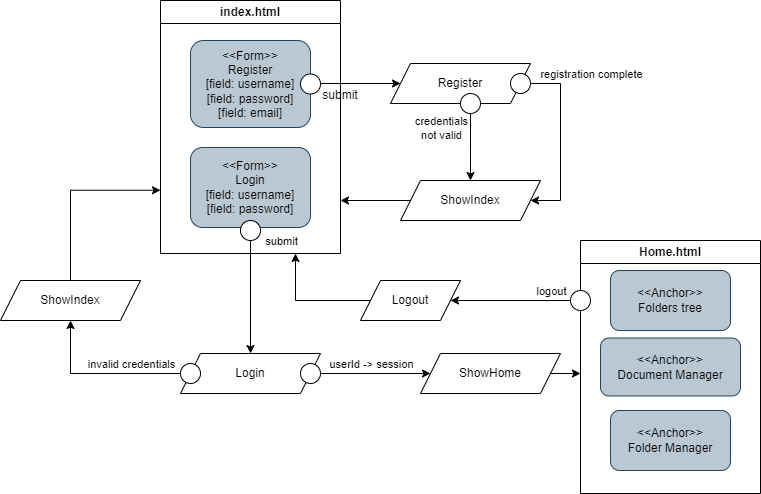
\includegraphics[width=0.9\textwidth]{HTML/HTMLLogin.png}
    \caption{Login and register.}
\end{figure}

\begin{figure}[H]
    \centering
    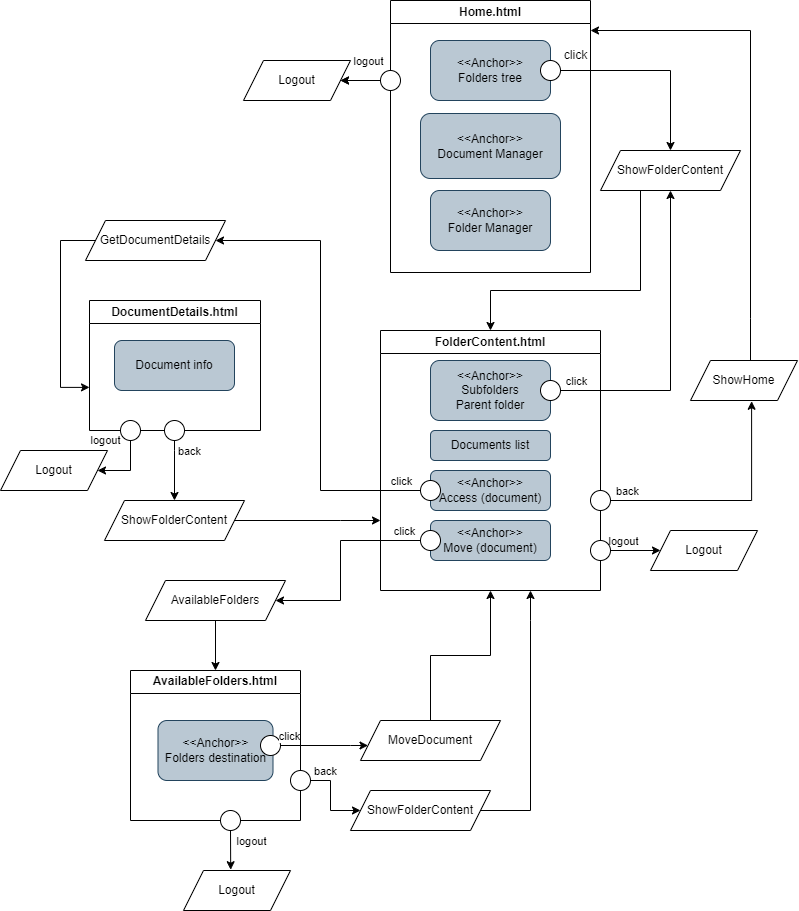
\includegraphics[width=0.9\textwidth]{HTML/HTMLDocumentAccessMove.png}
    \caption{Document access and move.}
\end{figure}

\begin{figure}[H]
    \centering
    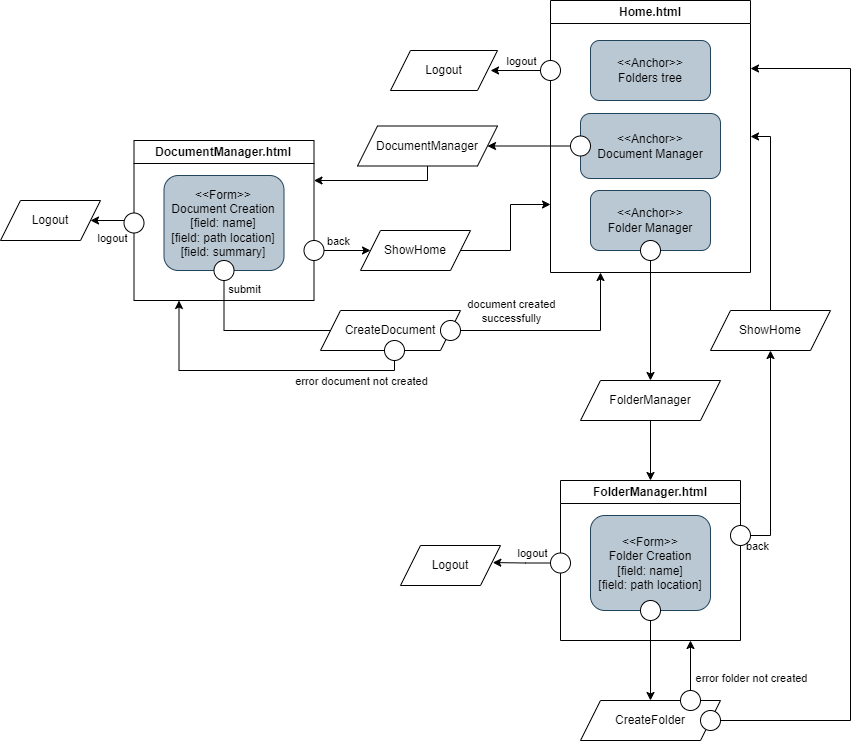
\includegraphics[width=0.9\textwidth]{HTML/HTMLFolderDocumentManager.png}
    \caption{Document manager. Folder manager.}
\end{figure}
\newpage

\myparagraph{Sequence diagrams}
Notes:
\begin{itemize} 
	\item{For the sake of keeping the diagram simple to understand, it's assumed that there is no ill-intentioned user, so only some exceptions are shown. Of course everything is checked and a proper error message is sent back if anything goes wrong.}
	\item{Operations such as establishing and closing the connection are not shown for the same reason.}
	\item{Documents with same name means they have the same name and the same format.}
	\item{Folders with same name means they just have the same name.}
\end{itemize}
\begin{figure}[H]
    \centering
    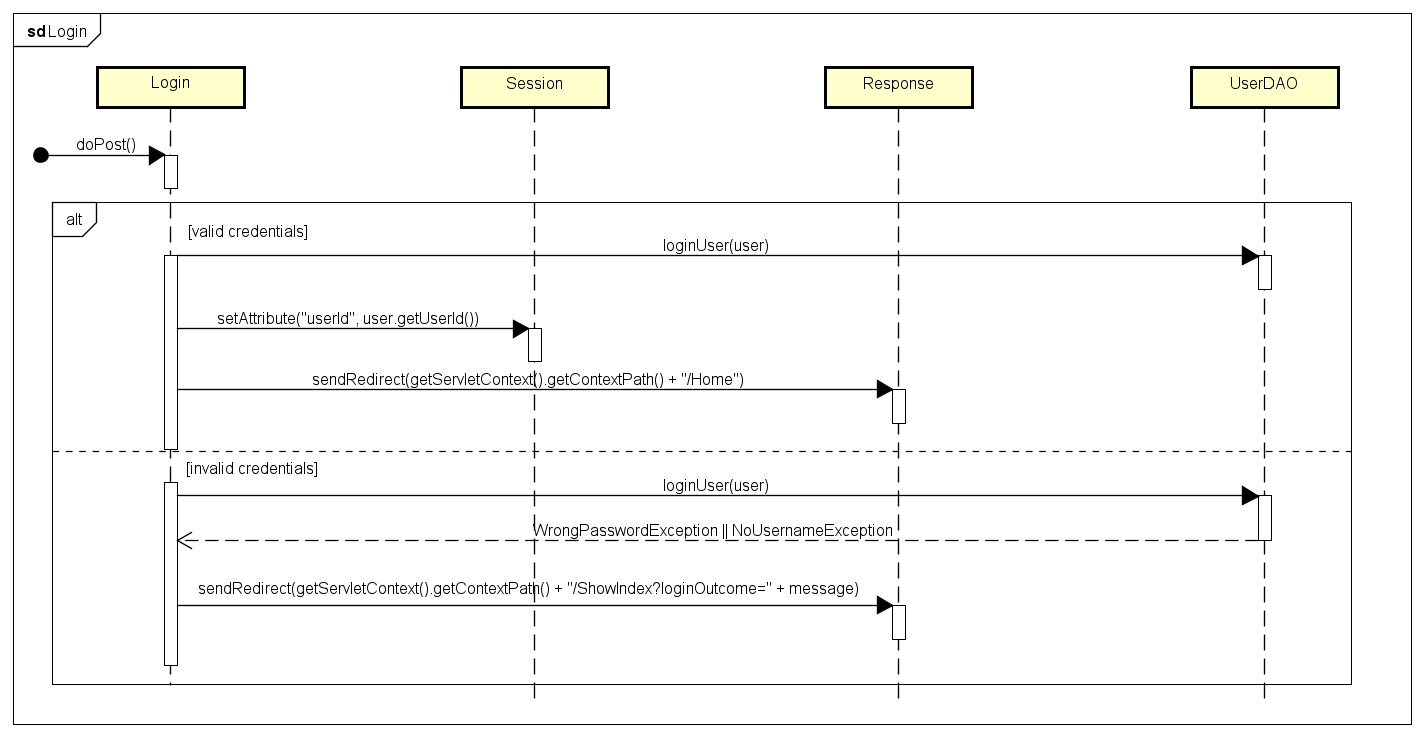
\includegraphics[width=1.0\textwidth]{HTML/SequenceDiagram/Login.png}
    \caption{Login sequence.}
\end{figure}

\begin{figure}[H]
    \centering
    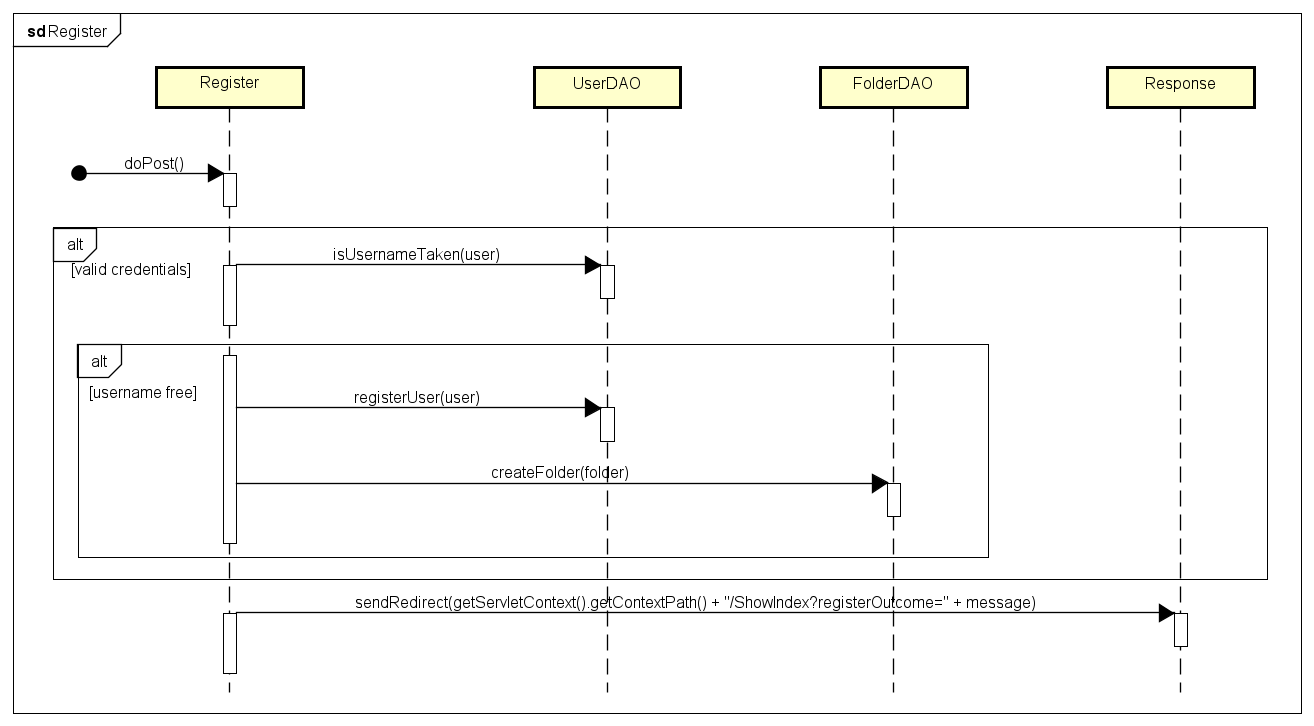
\includegraphics[width=1.0\textwidth]{HTML/SequenceDiagram/Register.png}
    \caption{Register sequence.}
\end{figure}
    
\begin{figure}[H]
    \centering
    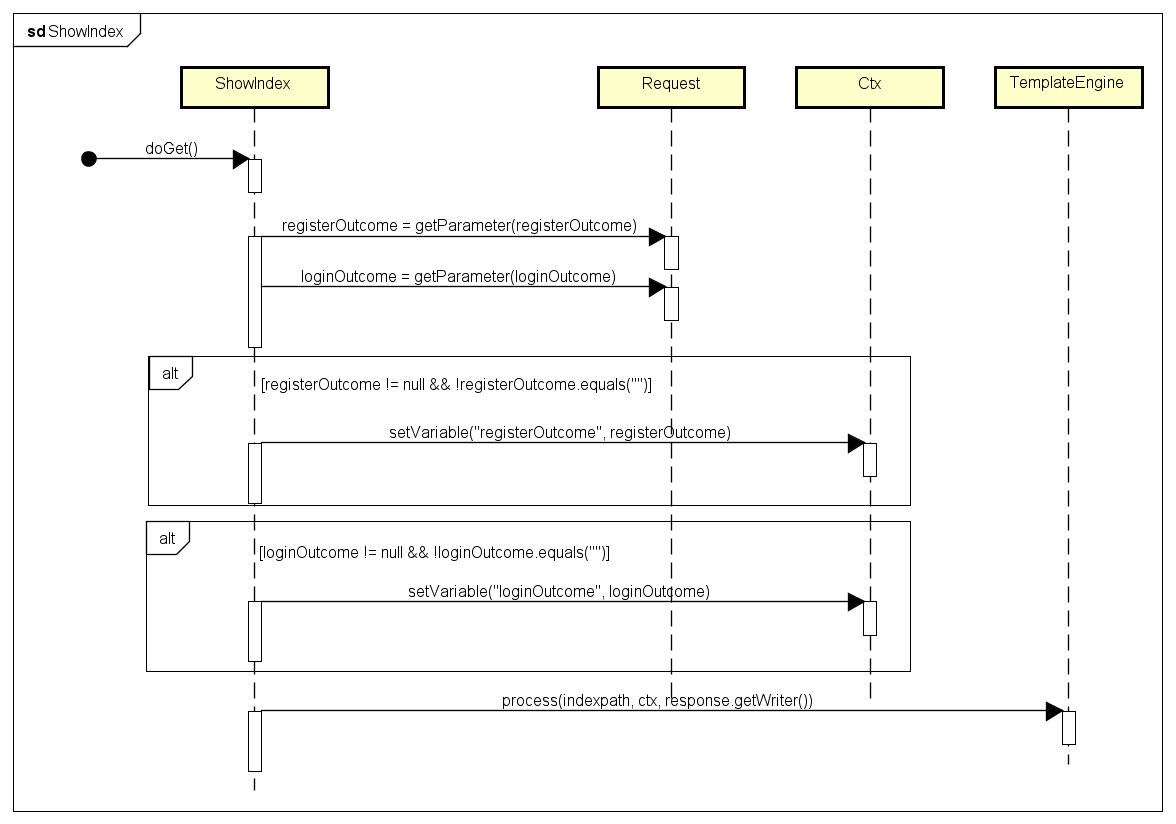
\includegraphics[width=1.0\textwidth]{HTML/SequenceDiagram/ShowIndex.png}
    \caption{Index messages sequence.}
\end{figure}

\begin{figure}[H]
    \centering
    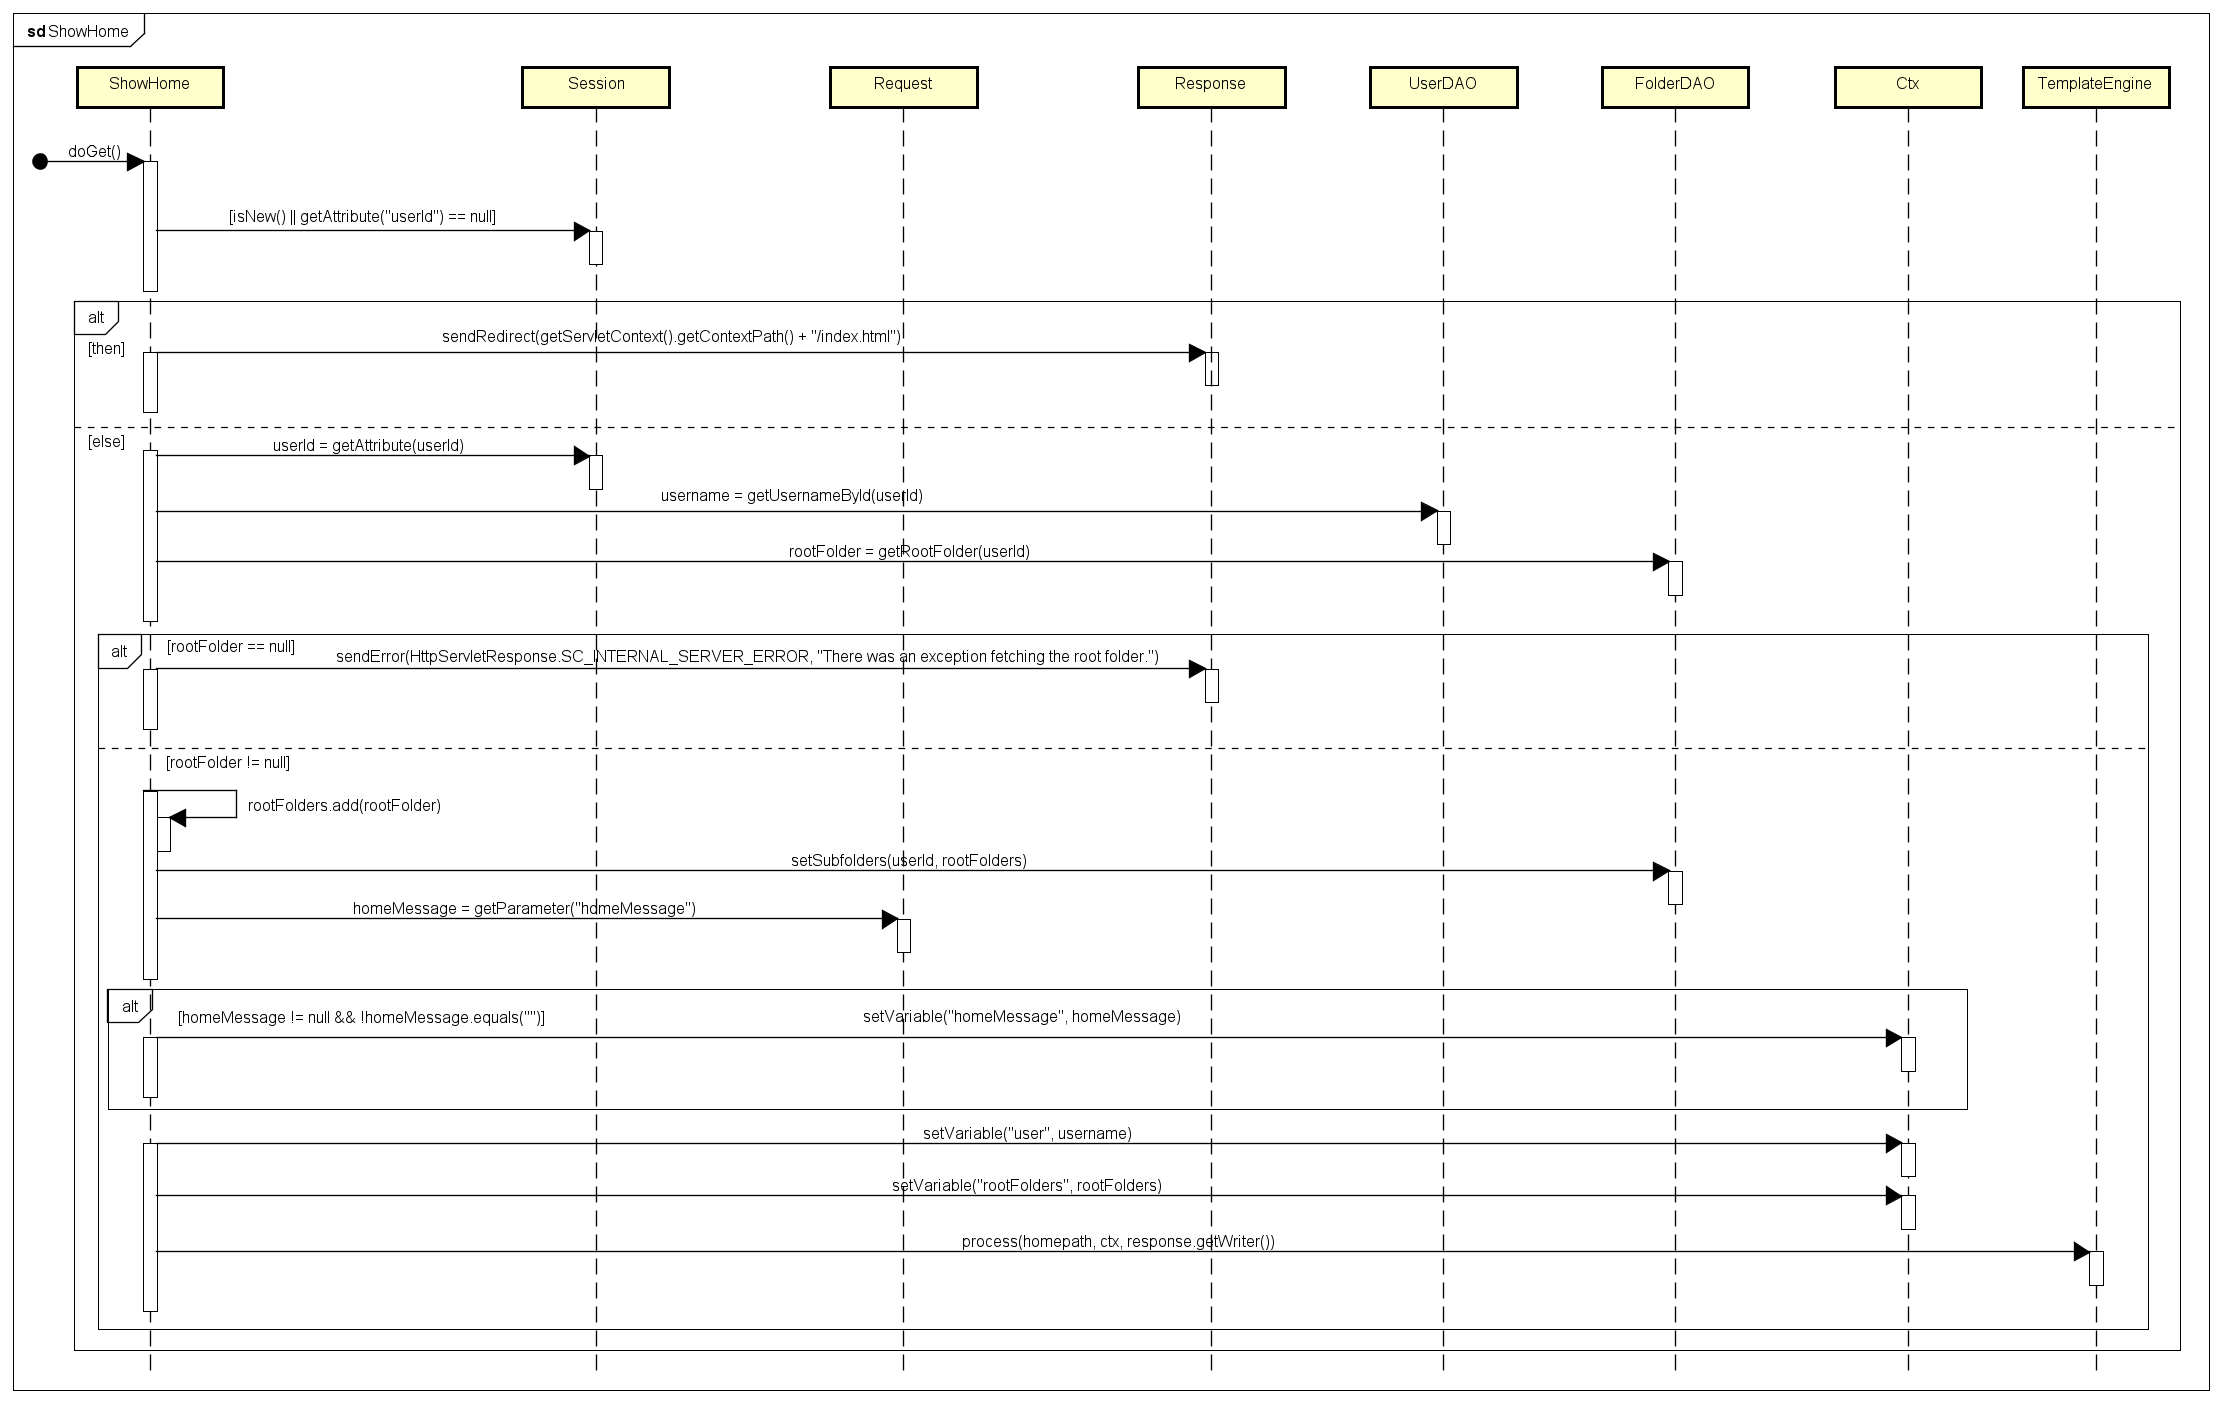
\includegraphics[width=1.0\textwidth]{HTML/SequenceDiagram/ShowHome.png}
    \caption{Home page sequence.}
\end{figure}

\begin{figure}[H]
    \centering
    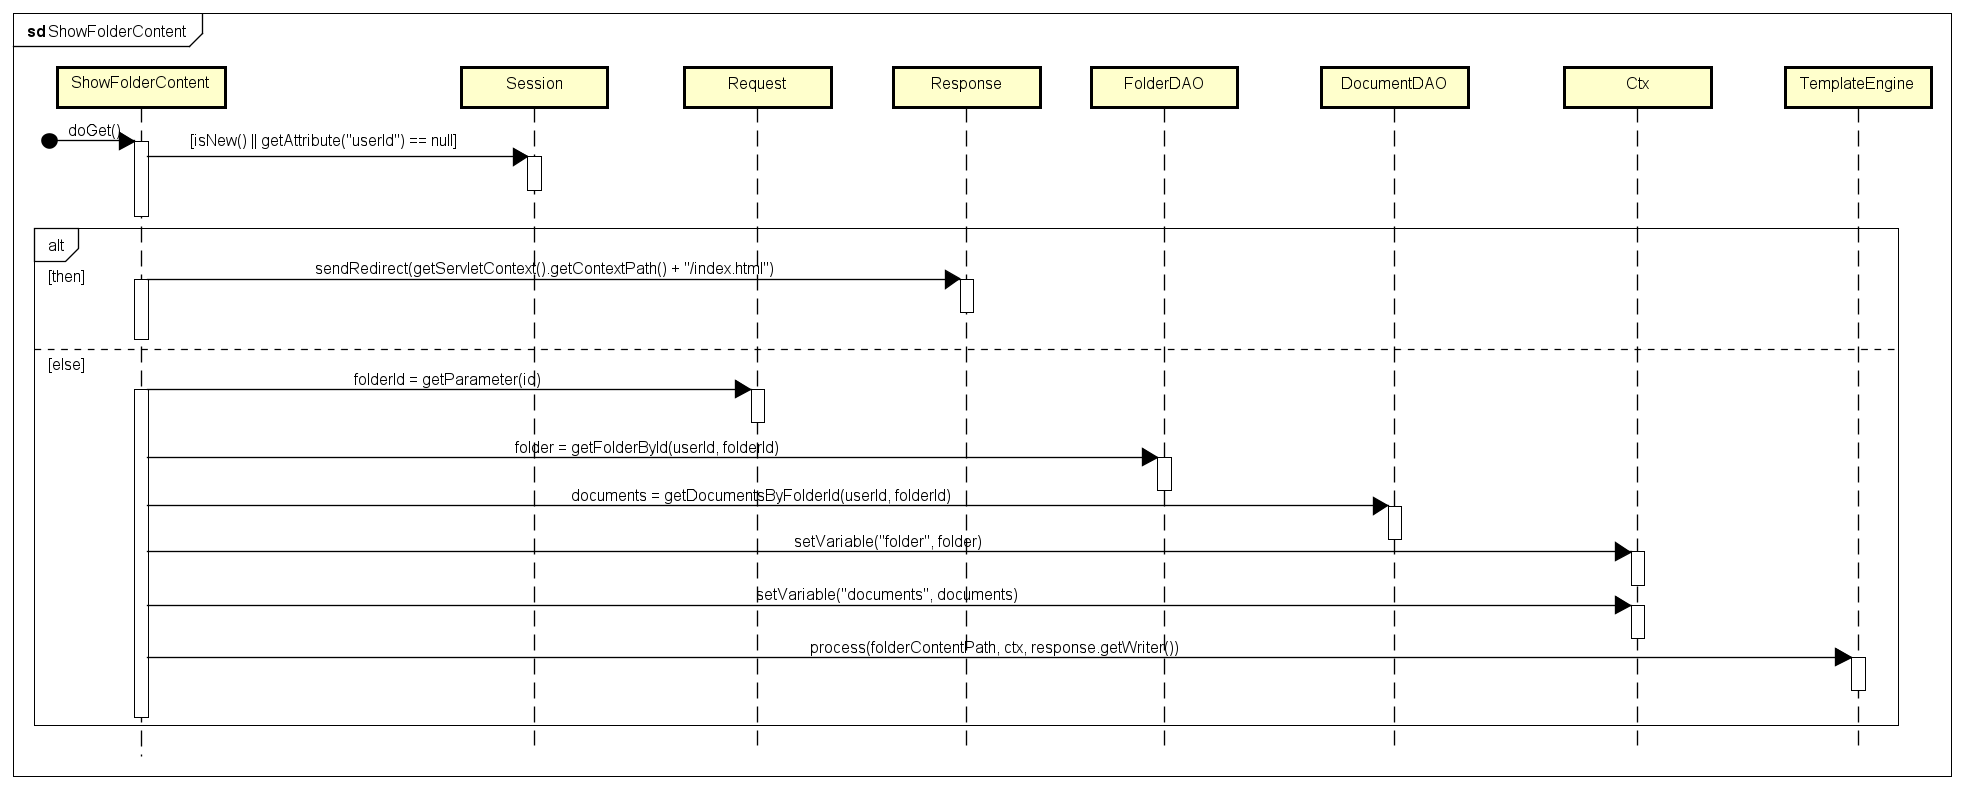
\includegraphics[width=1.0\textwidth]{HTML/SequenceDiagram/ShowFolderContent.png}
    \caption{Accessing a folder sequence.}
\end{figure}
    
\begin{figure}[H]
    \centering
    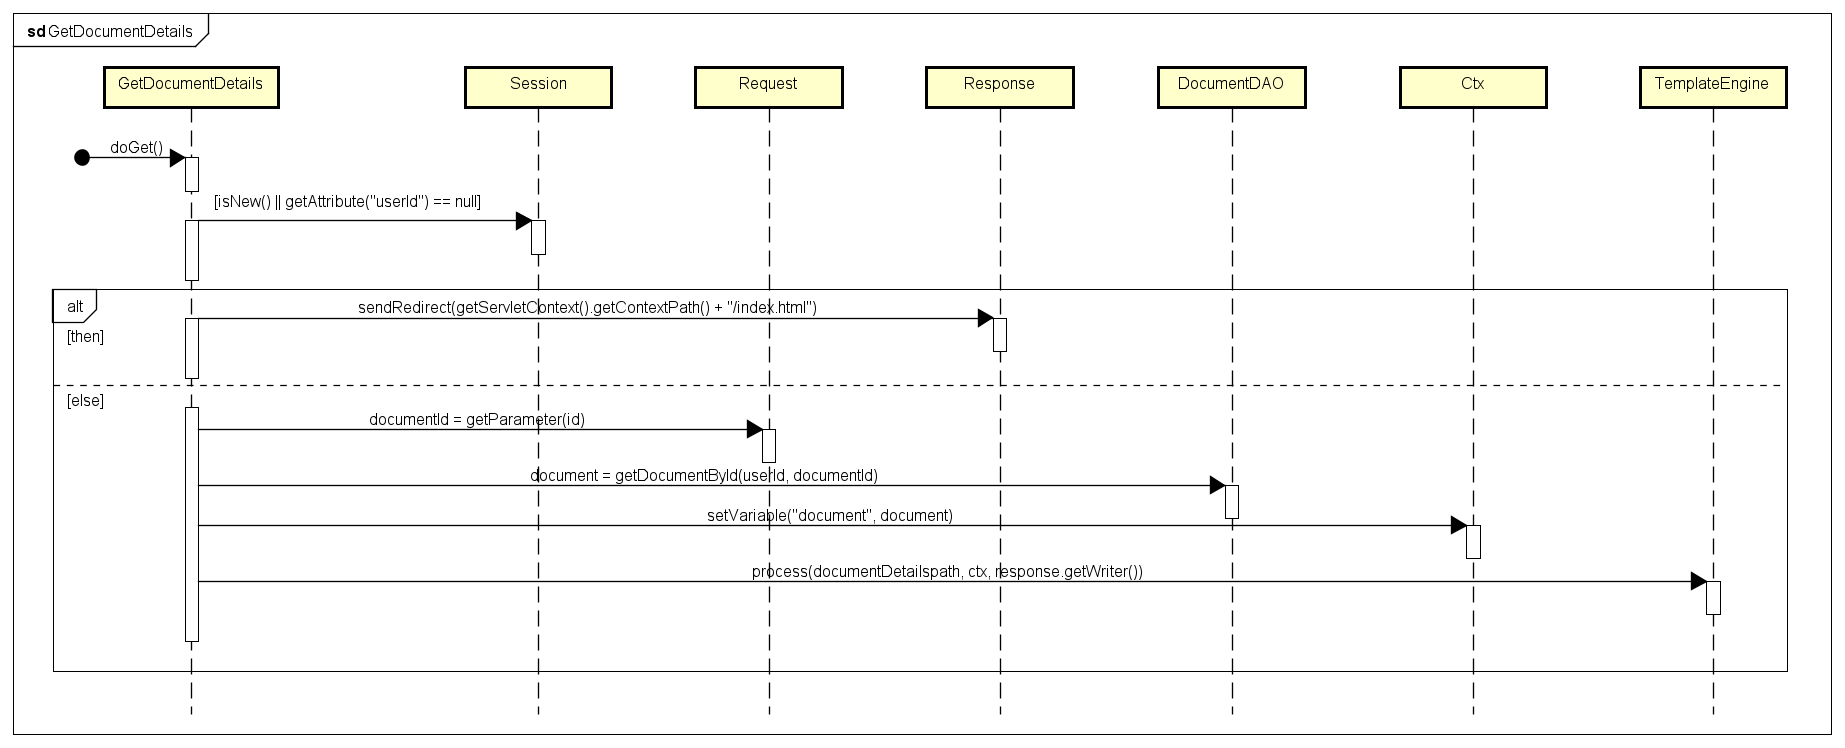
\includegraphics[width=1.0\textwidth]{HTML/SequenceDiagram/GetDocumentDetails.png}
    \caption{Accessing a document's details sequence.}
\end{figure}

\begin{figure}[H]
    \centering
    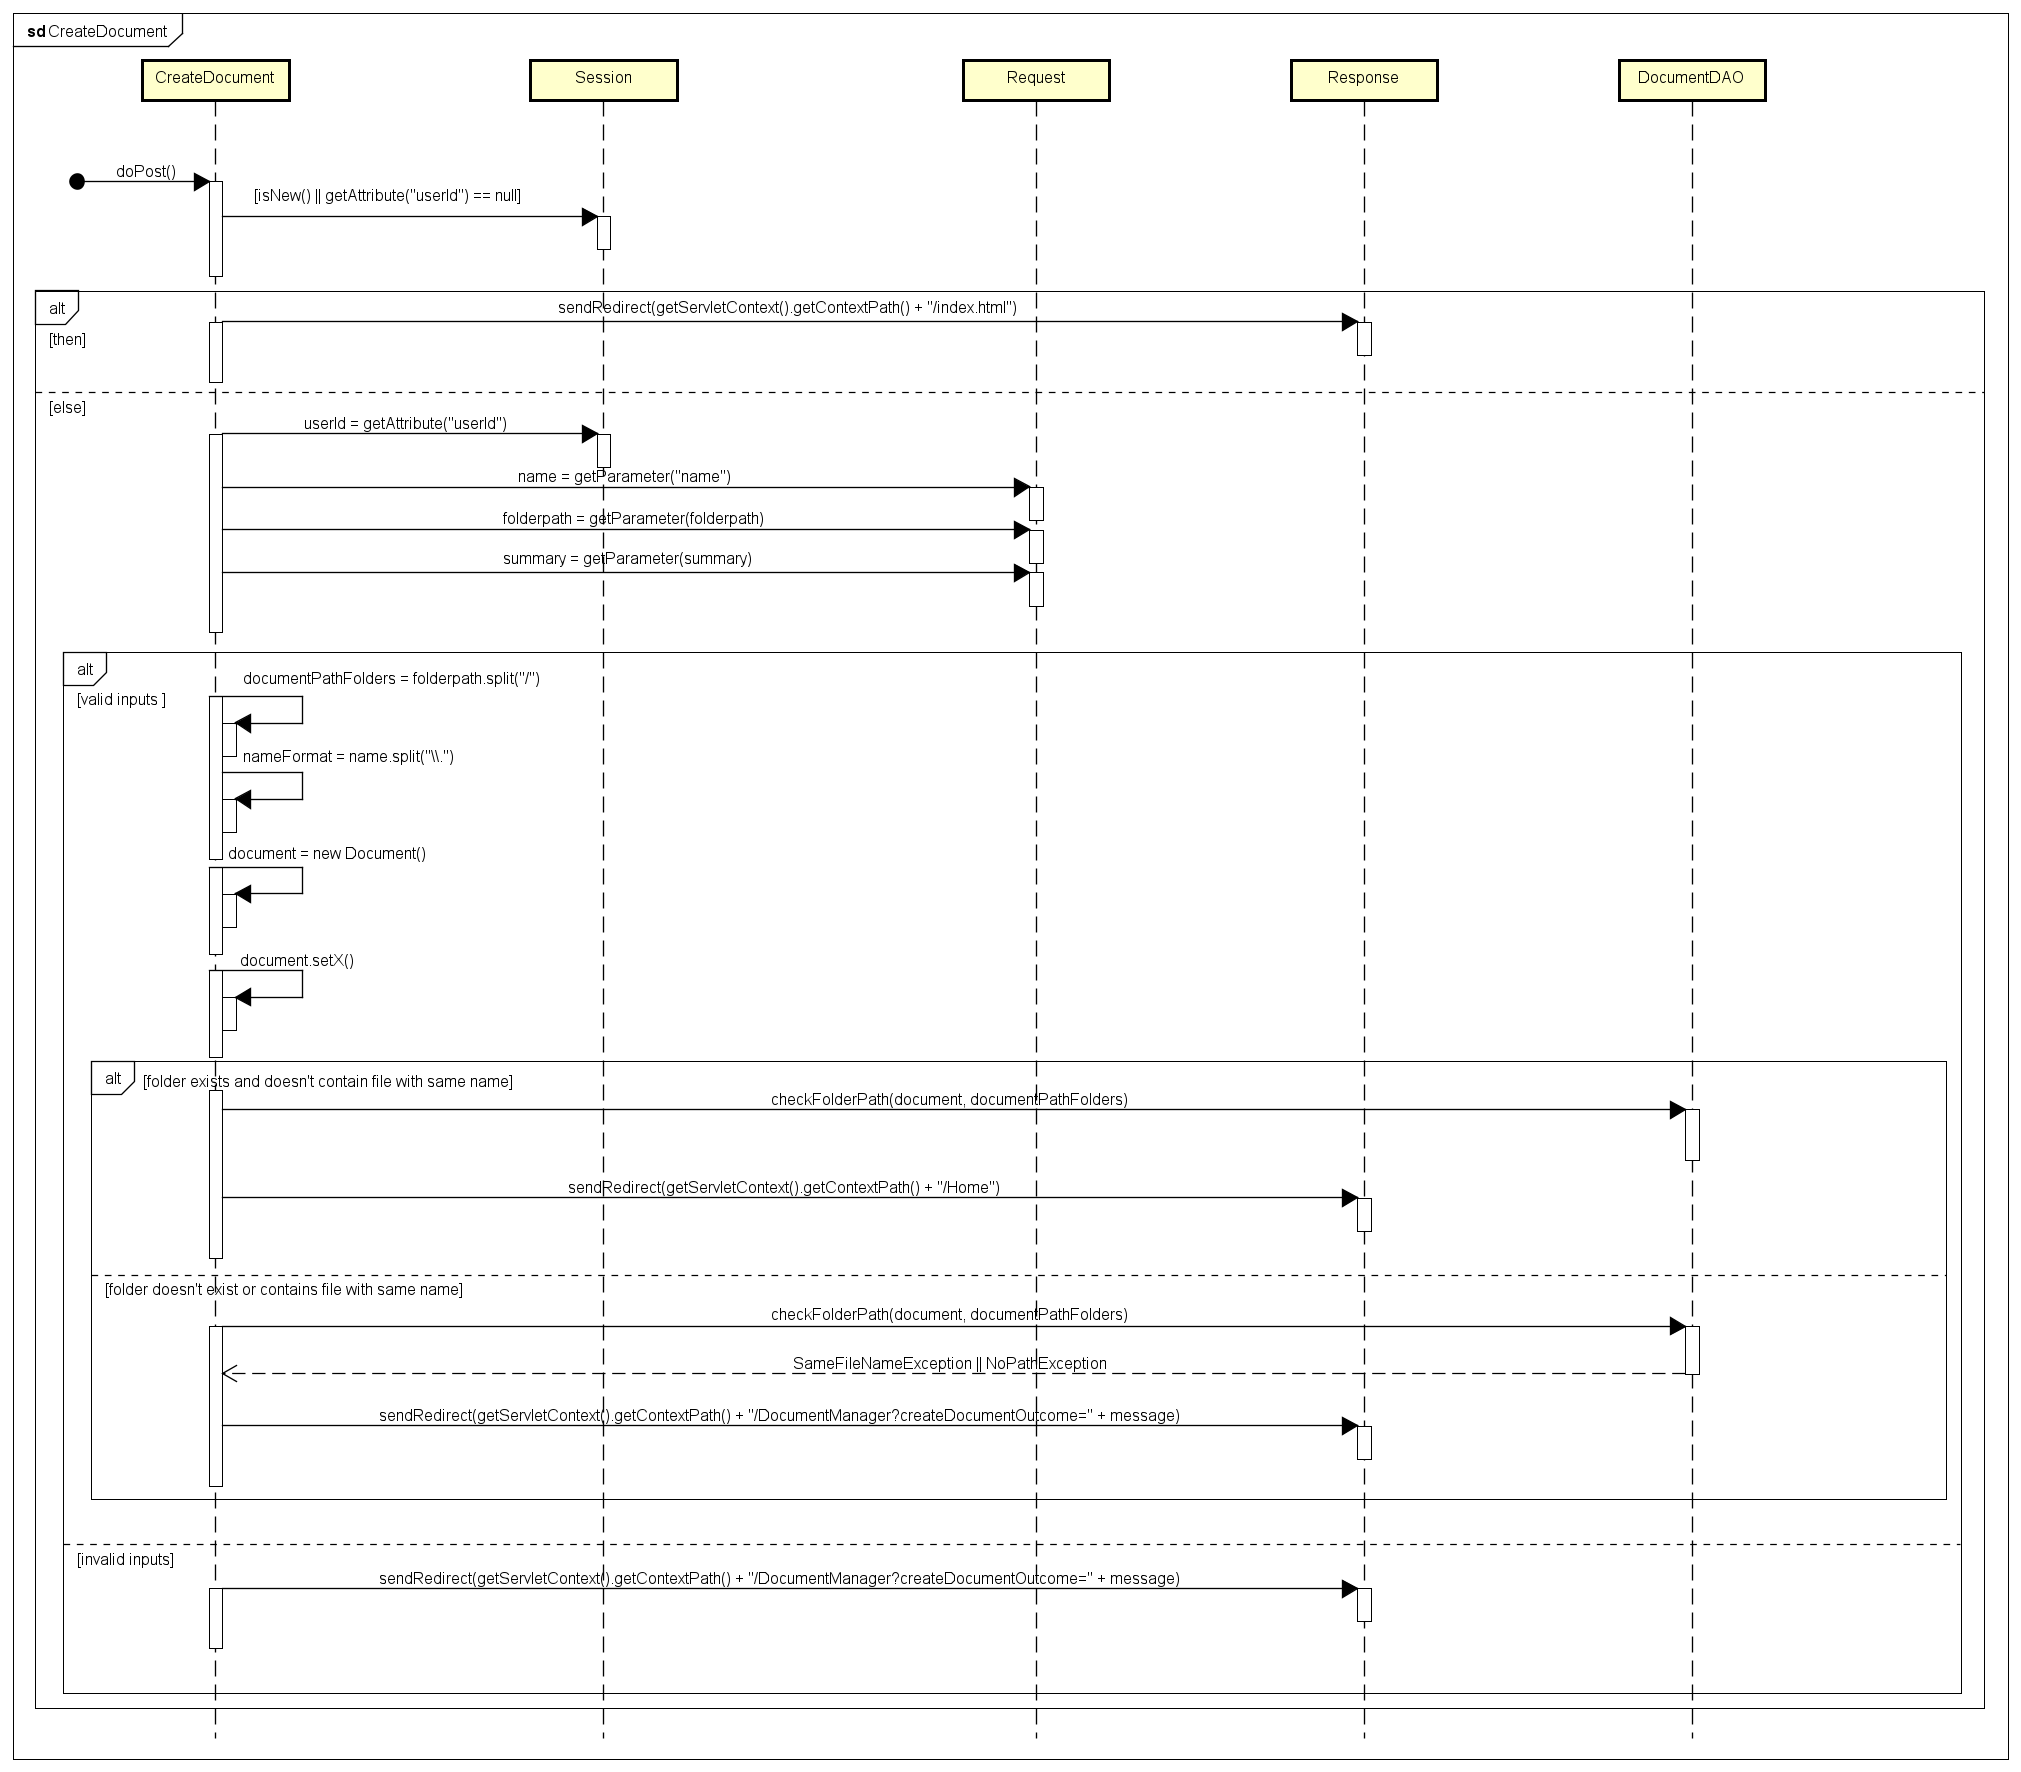
\includegraphics[width=1.0\textwidth]{HTML/SequenceDiagram/CreateDocument.png}
    \caption{Creating a document sequence.}
\end{figure}
    
\begin{figure}[H]
    \centering
    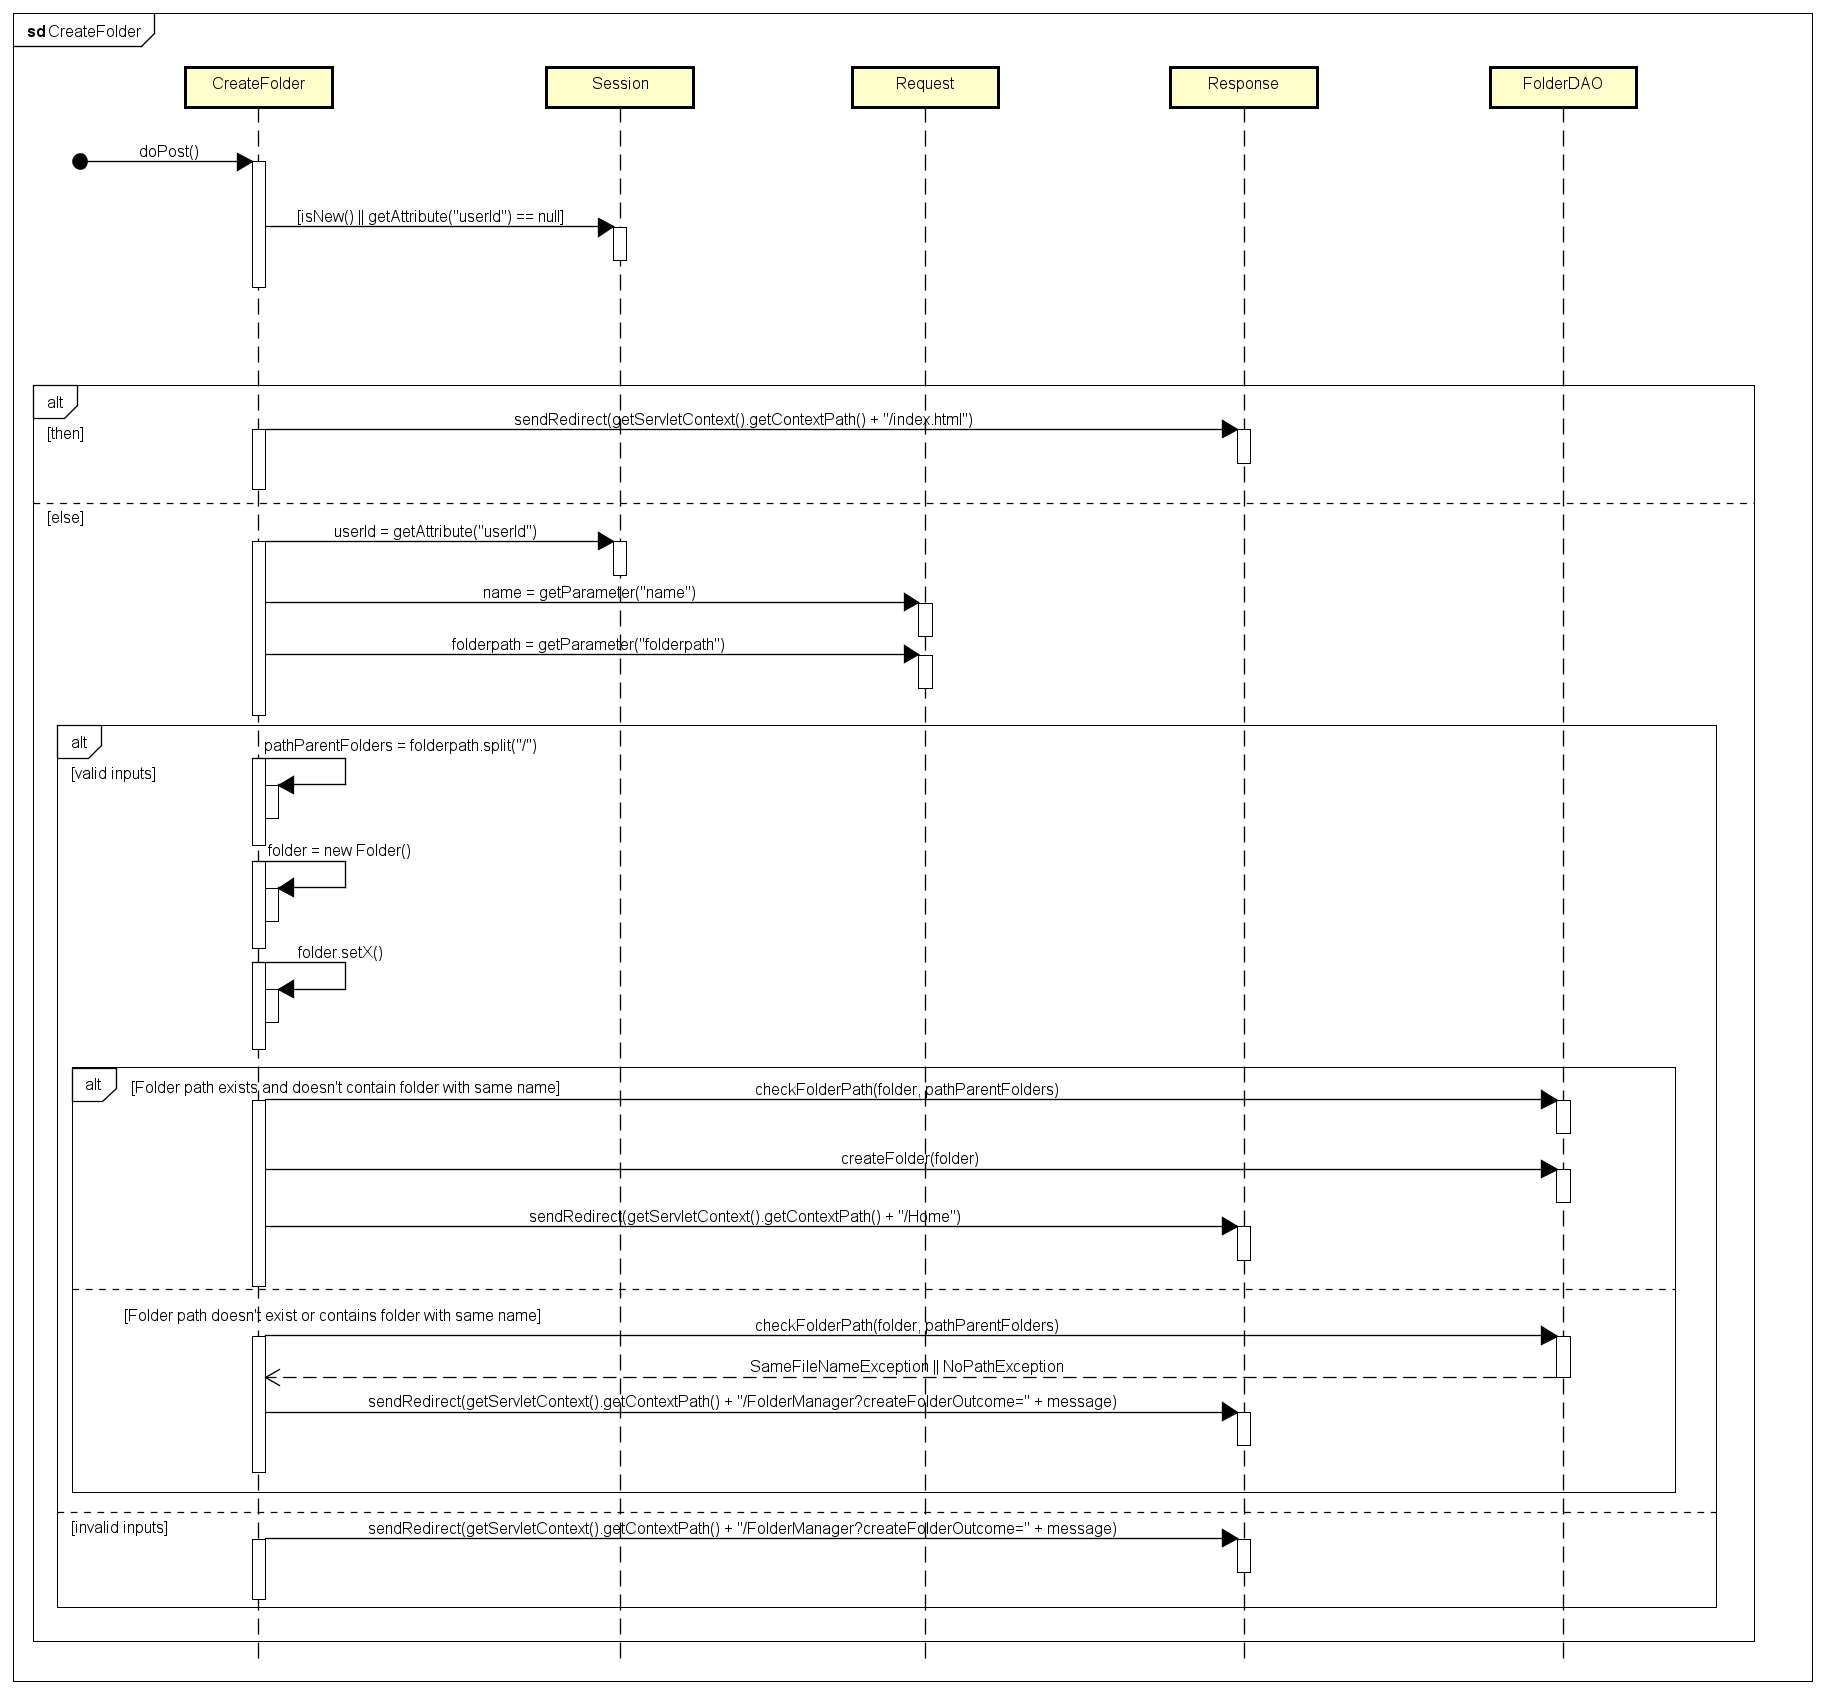
\includegraphics[width=1.0\textwidth]{HTML/SequenceDiagram/CreateFolder.png}
    \caption{Creating a folder sequence.}
\end{figure}
    
\begin{figure}[H]
    \centering
    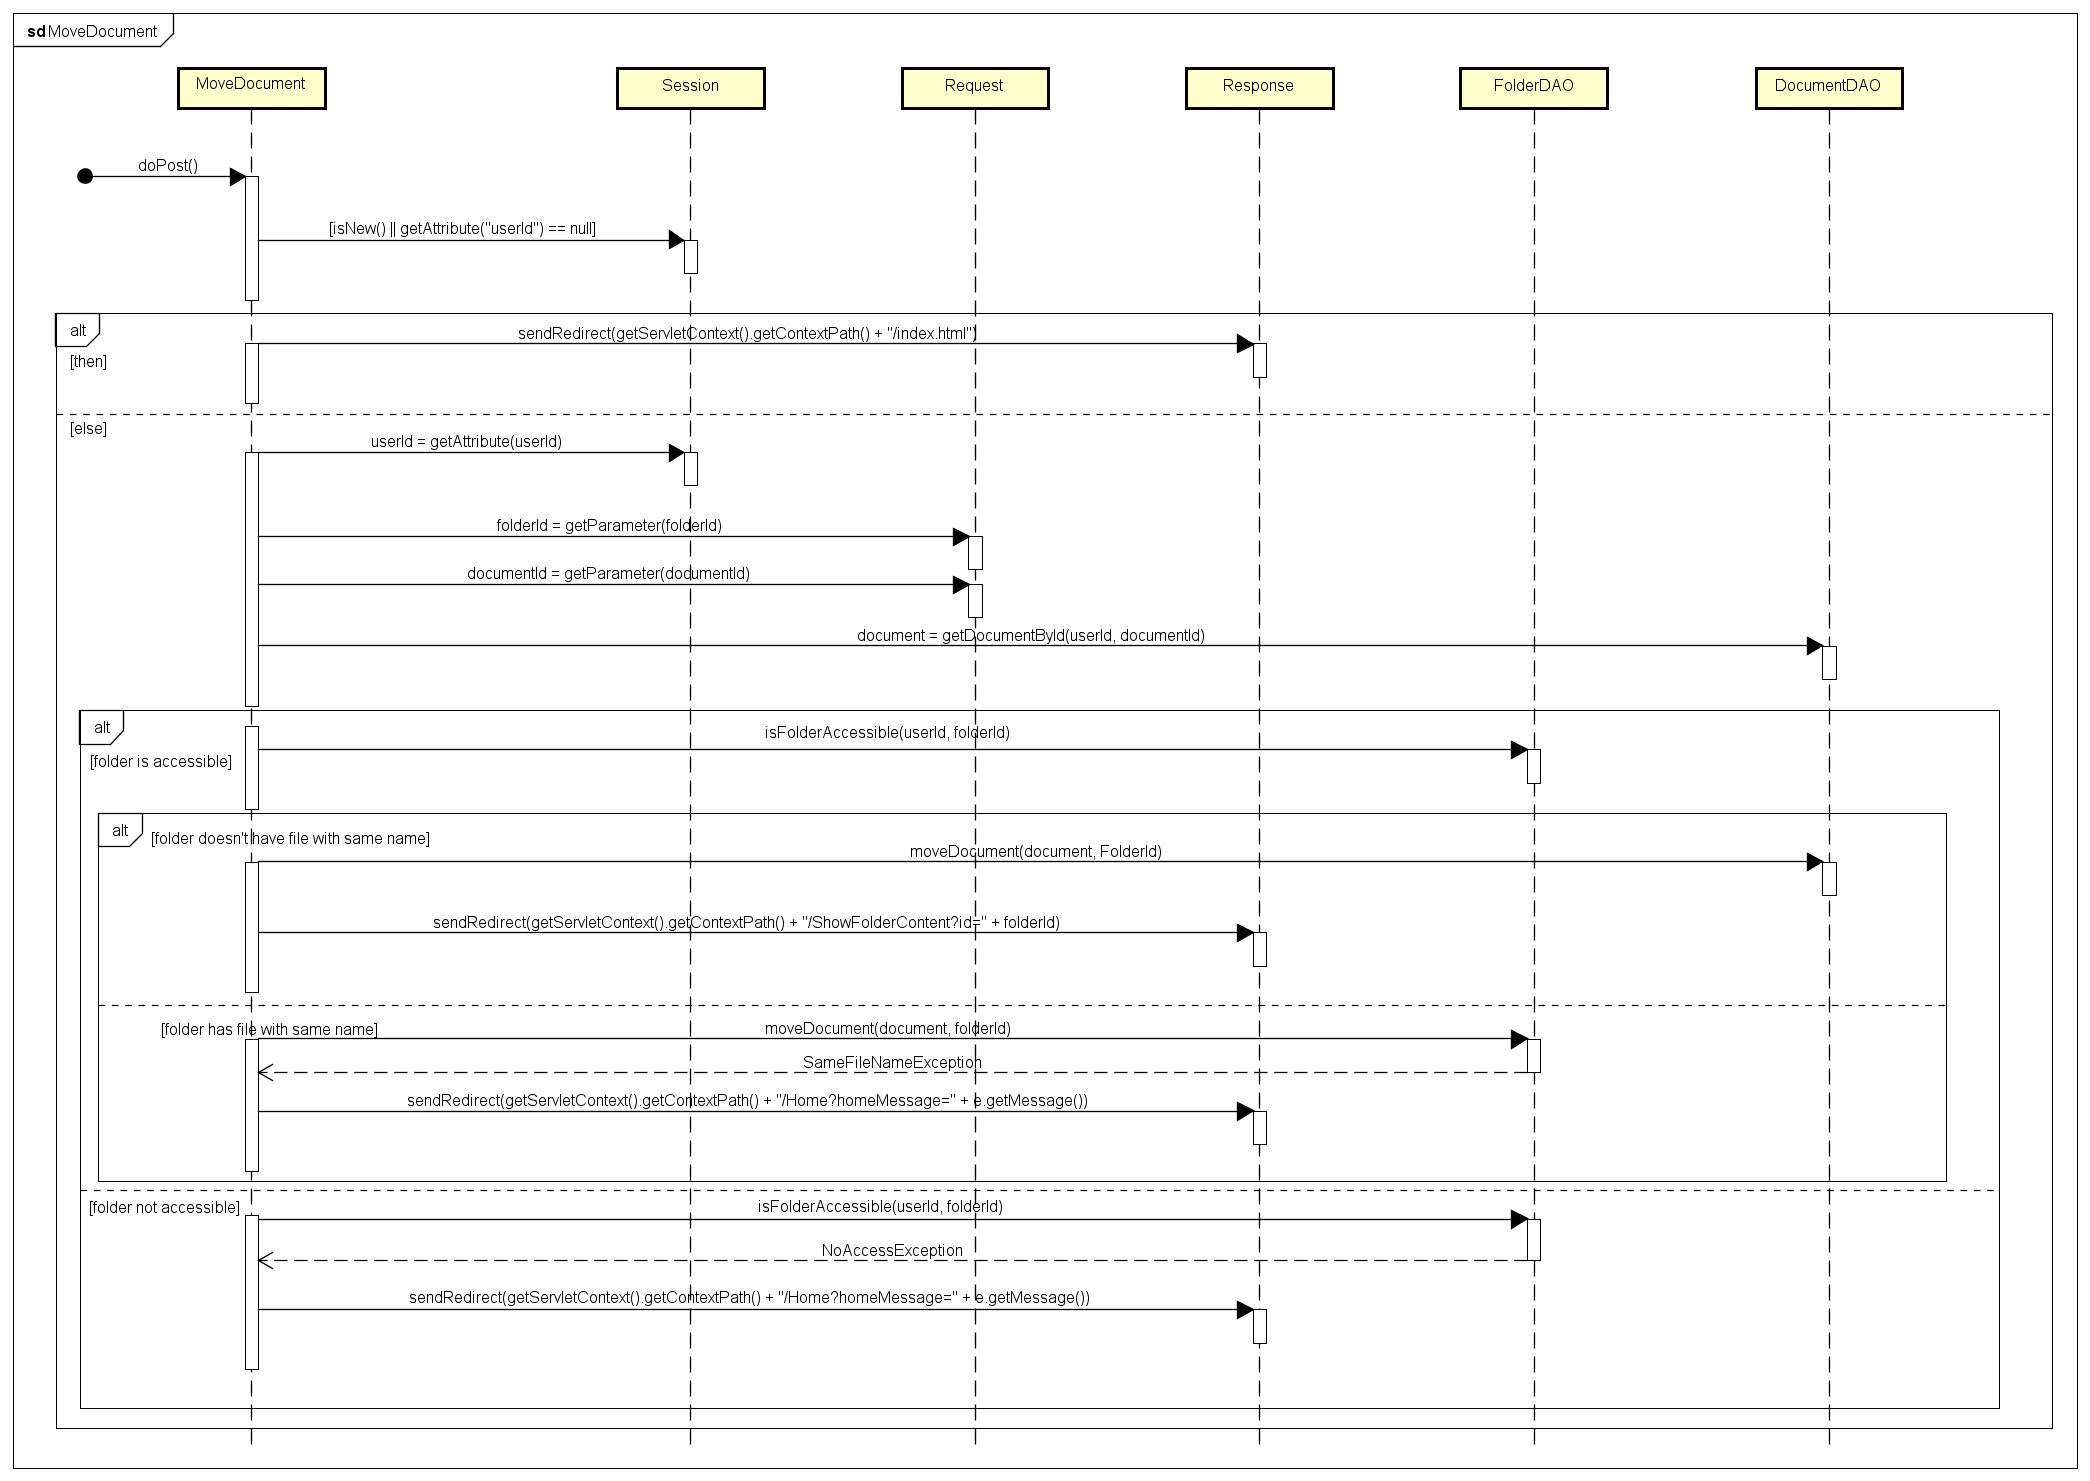
\includegraphics[width=1.0\textwidth]{HTML/SequenceDiagram/MoveDocument.png}
    \caption{Moving a document sequence.}
\end{figure}
    
\newpage

\section{JavaScript version}
\subsection{Project analysis}
\paragraph{Application requirements}
[\textcolor{darkred}{Pages} \textcolor{darkgreen}{View components} \textcolor{darkblue}{Events} \textcolor{darkyellow}{Actions}]\\
The application still supports \textcolor{blue}{login and registration} via \textcolor{darkgreen}{forms}, and in addition to the \textcolor{darkyellow}{syntax validation of the email}, the \textcolor{darkyellow}{equality of the "password" and "repeat password" fields is also checked} on the client and server side. After the user logs in, the entire application is implemented on a \textcolor{darkred}{single page}. \textcolor{darkgreen}{Error messages} are displayed within the page for the user to see. The \textcolor{darkyellow}{movement of documents or folders} occurs via \textcolor{darkblue}{drag and drop}. Next to each folder, \textcolor{darkgreen}{two labeled buttons appear "add subfolder" and "add document"}, they respectively \textcolor{darkyellow}{trigger a form} to \textcolor{darkblue}{input the name of the subfolder or the document details}. Finally, a \textcolor{darkgreen}{folder called "trash bin"} is added; \textcolor{darkblue}{dragging a document into the trash} results in \textcolor{darkyellow}{its deletion}. Before deleting the document, a \textcolor{darkgreen}{confirmation window appears}. \textcolor{darkyellow}{Deleting a folder results in the complete and recursive deletion of all data (documents and subfolders)}.

\paragraph{Additional notes}
Beside the login, the application core functions work on a single homepage and the content refreshes without the use of the browser's refresh button (Single Page Architecture). Both the client-side and server-side must check the validity of the user's inputs. The server doesn't expose its core functions, instead the client's side JavaScript has to make use of the function makecall(). All objects returned from the server are JSON. 
\newpage
\subsection{Project design}
\myparagraph{Components}
\begin{multicols}{2}
Beans (Java)
\begin{itemize}
	\item{Document}
	\item{Folder}
	\item{User}
\end{itemize}
Data Access Objects (Java)
\begin{itemize}
	\item{DocumentDao}
	\begin{itemize}
		\item{createDocument}
		\item{checkDocumentFolderChildren}
		\item{getDocumentsByFolderId}
		\item{getDocumentById}
		\item{addDocumentsToFolder}
		\item{getDocumentByParameters}
		\item{isDocumentAccessible}
		\item{moveDocument}
		\item{deleteDocument}
	\end{itemize}
	\item{FolderDao}
	\begin{itemize}
		\item{getRootFolder}
		\item{setSubFolders}
		\item{createFolder}
		\item{checkParentFolderChildren}
		\item{isFolderAccessible}
		\item{getFolderByParameters}
		\item{getFolderById}
		\item{isFolderRoot}
		\item{deleteFolder}
	\end{itemize}
	\item{UserDao}
	\begin{itemize}
		\item{getUsernameById}
		\item{loginUser}
		\item{registerUser}
		\item{isUsernameTaken}
	\end{itemize}
\end{itemize}
Views (HTML)
\begin{itemize}
	\item{index (page showing the log in and register forms)}
	\item{Home (page showing the tree of folders, documents and server messages)}
\end{itemize}
Controllers (Java)
\begin{itemize}
	\item{CheckLogin}
	\item{CheckRegister}
	\item{CreateDocument}
	\item{CreateFolder}
	\item{DeleteDocument}
	\item{DeleteFolder}
	\item{GetFolders}
	\item{Logout}
	\item{MoveDocument}
\end{itemize}
\end{multicols}
Note: because of the change in the application's structure, the Folder bean had to be modified. Subfolders and documents parameters have been added to it, so that on homepage's load the entire structure could be saved on the client's side.
\newpage 

\paragraph{Activity diagrams}\mbox{}

\begin{figure}[H]
    \centering
    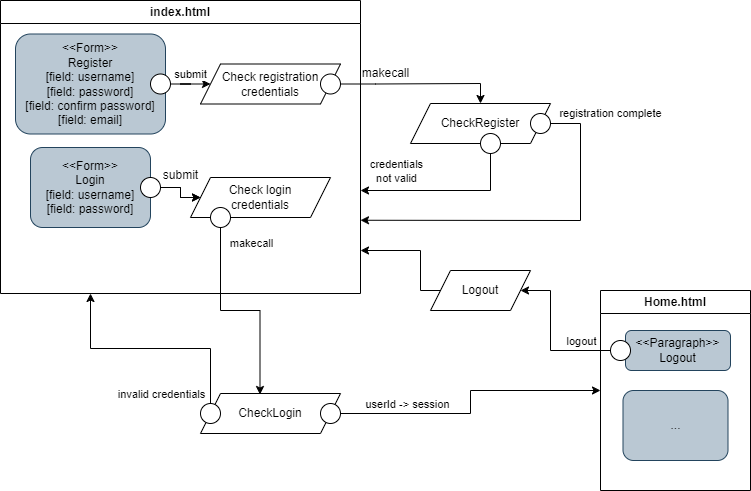
\includegraphics[width=0.9\textwidth]{JS/JSLoginSequence.png}
    \caption{Login and register.}
\end{figure}
\begin{figure}[H]
    \centering
    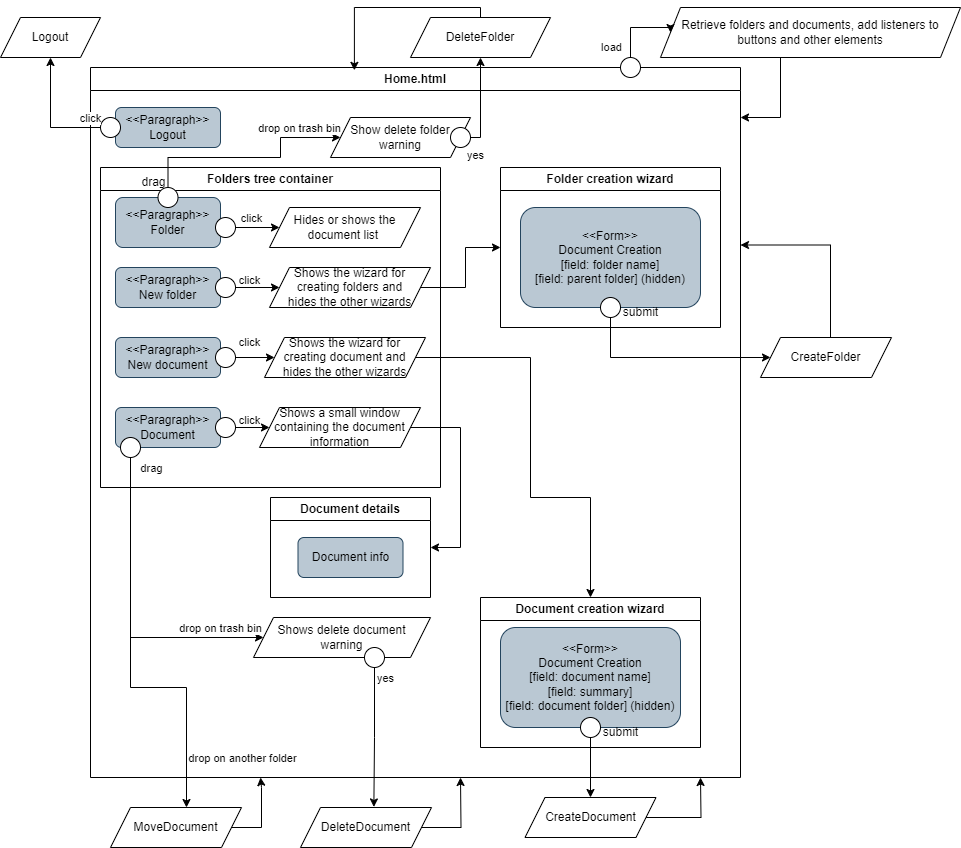
\includegraphics[width=0.9\textwidth]{JS/JSHomeSequence.png}
    \caption{Home.}
\end{figure}

\newpage
\paragraph{Events and actions}
Note: for the sake of keeping it short, most of the checks are omitted, obviously everything is checked and if something is wrong the user gets an error message. If the session has expired the user is kicked out and sent to the index page.
\begin{center}
\begin{tabular}{|p{4cm}|p{4cm}|p{4cm}|p{4cm}|}
\hline

\multicolumn{2}{|c|}{\textbf{Client side}} & \multicolumn{2}{c|}{\textbf{Server side}}\\
\hline
\textbf{Event} & \textbf{Action} & \textbf{Event} & \textbf{Action} \\
\hline 
index $\rightarrow$ login form $\rightarrow$ submit & Check form fields & POST (username, password) & Credentials check \\
\hline 
index $\rightarrow$ register form $\rightarrow$ submit & Check form fields & POST (username, password, confirmPassword, email) & Credentials check and root folder creation\\
\hline  
Home page $\rightarrow$ load & Updates the page with folders tree (without refreshing the entire page) & GET () & Retrieve all the folders for the user in a tree structure\\
\hline
Home page $\rightarrow$ click on a folder & Show the list of documents under the folder & &\\
\hline
Home page $\rightarrow$ click on a document & Show the details of the document & &\\
\hline
Home page $\rightarrow$ click on logout & & GET () & Log out the user and send to index\\
\hline
Home page $\rightarrow$ click on new folder $\rightarrow$ submit & Show the wizard $\rightarrow$ check form fields & POST (folderName, parentFolderId) & Create a new subfolder in the parent folder\\
\hline
Home page $\rightarrow$ click on new document $\rightarrow$  submit & Show the wizard $\rightarrow$ check form fields & POST (documentName, summary, documentFolderId) & Create a new document in the folder\\
\hline
Home page $\rightarrow$  drag document $\rightarrow$  drop on a folder & & POST (documentId, targetFolderId) & Move the document to the specified folder\\
\hline
Home page $\rightarrow$ drag document $\rightarrow$ drop on trash bin $\rightarrow$ confirm & Show the warning box for document deletion & POST (documentId) & Delete the specified document\\
\hline
Home page $\rightarrow$ drag folder $\rightarrow$ drop on trash bin $\rightarrow$ confirm & Show the warning box for folder deletion & POST (folderId) & Delete the specified folder and the subfolders recursively\\
\hline
\end{tabular}
\end{center}
\newpage

\begin{center}
\begin{tabular}{|p{4cm}|p{4cm}|p{4cm}|p{4cm}|}
\hline

\multicolumn{2}{|c|}{\textbf{Client side}} & \multicolumn{2}{c|}{\textbf{Server side}}\\
\hline
\textbf{Event} & \textbf{Controller (function)} & \textbf{Event} & \textbf{Controller (servlet)} \\
\hline
index $\rightarrow$ login form $\rightarrow$ submit & makeCall () & POST (username, password) & CheckLogin\\
\hline
index $\rightarrow$ register form $\rightarrow$ submit & makeCall () & POST (username, password, confirmPassword, email) & CheckRegister\\
\hline
Home page $\rightarrow$ load & pageOrchestrator.start (), FoldersTree.get (), buildFoldersTree (), makeCall () & GET () & GetFolders\\
\hline
Home page $\rightarrow$ refresh (after adding or removing files) & pageOrchestrator. refresh (), FoldersTree.refresh (), buildFoldersTree () & &\\
\hline
Home page $\rightarrow$ click on a folder & & &\\ 
\hline
Home page $\rightarrow$ click on a document & & &\\
\hline
Home page $\rightarrow$  click on logout & pageOrchestrator () & GET() & Logout\\
\hline
Home page $\rightarrow$ click on new folder $\rightarrow$ submit & subfolderWizard (), makeCall () & POST (folderName, parentFolderId) & CreateFolder\\
\hline
Home page $\rightarrow$ click on new document $\rightarrow$ submit & documentWizard (), makeCall () & POST (documentName, summary, documentFolderId) & CreateDocument\\
\hline
Home page $\rightarrow$ drag document $\rightarrow$ drop on a folder & requestMoveDocument (), makeCall () & POST (documentId, targetFolderId) & MoveDocument\\
\hline
Home page $\rightarrow$ drag document $\rightarrow$ drop on trash bin $\rightarrow$ confirm & deleteDocumentAlert (), makeCall() & POST (documentId) & DeleteDocument\\
\hline
Home page $\rightarrow$ drag folder $\rightarrow$ drop on trash bin $\rightarrow$ confirm & deleteFolderAlert (), makeCall () & POST (folderId) & DeleteFolder\\
\hline

\end{tabular}
\end{center}
\newpage
\myparagraph{Sequence diagrams}
Notes:
\begin{itemize} 
	\item{For the sake of keeping the diagram simple to understand, it's assumed that there is no ill-intentioned user, so only some exceptions are shown. Of course everything is checked and a proper error message is sent back if anything goes wrong.}
	\item{Operations such as establishing and closing the connection are not shown for the same reason.}
	\item{Session tracking sequence isn't shown for the same reason, obviously if the user's session expired they get redirected to the index page.}
	\item{Documents with same name means they have the same name and the same format.}
	\item{Folders with same name means they just have the same name.}
	\item{Client side Javascript files are: fileManagementHome.js, loginManagement.js, registerManagement.js, utils.js. This last one contains the function makeCall() to do AJAX requests. Which will not be shown, using instead AJAX POST or AJAX GET for brevity. [C] means it's client-side while [S] is server-side.}
	\item{Folder deletion was done with setAutoCommit(false) in order to delete the folder, the documents and the subfolders safely. The application doesn't have to delete the files manually as the DB tables are set with ON DELETE CASCADE.}
\end{itemize}

\begin{figure}[H]
    \centering
     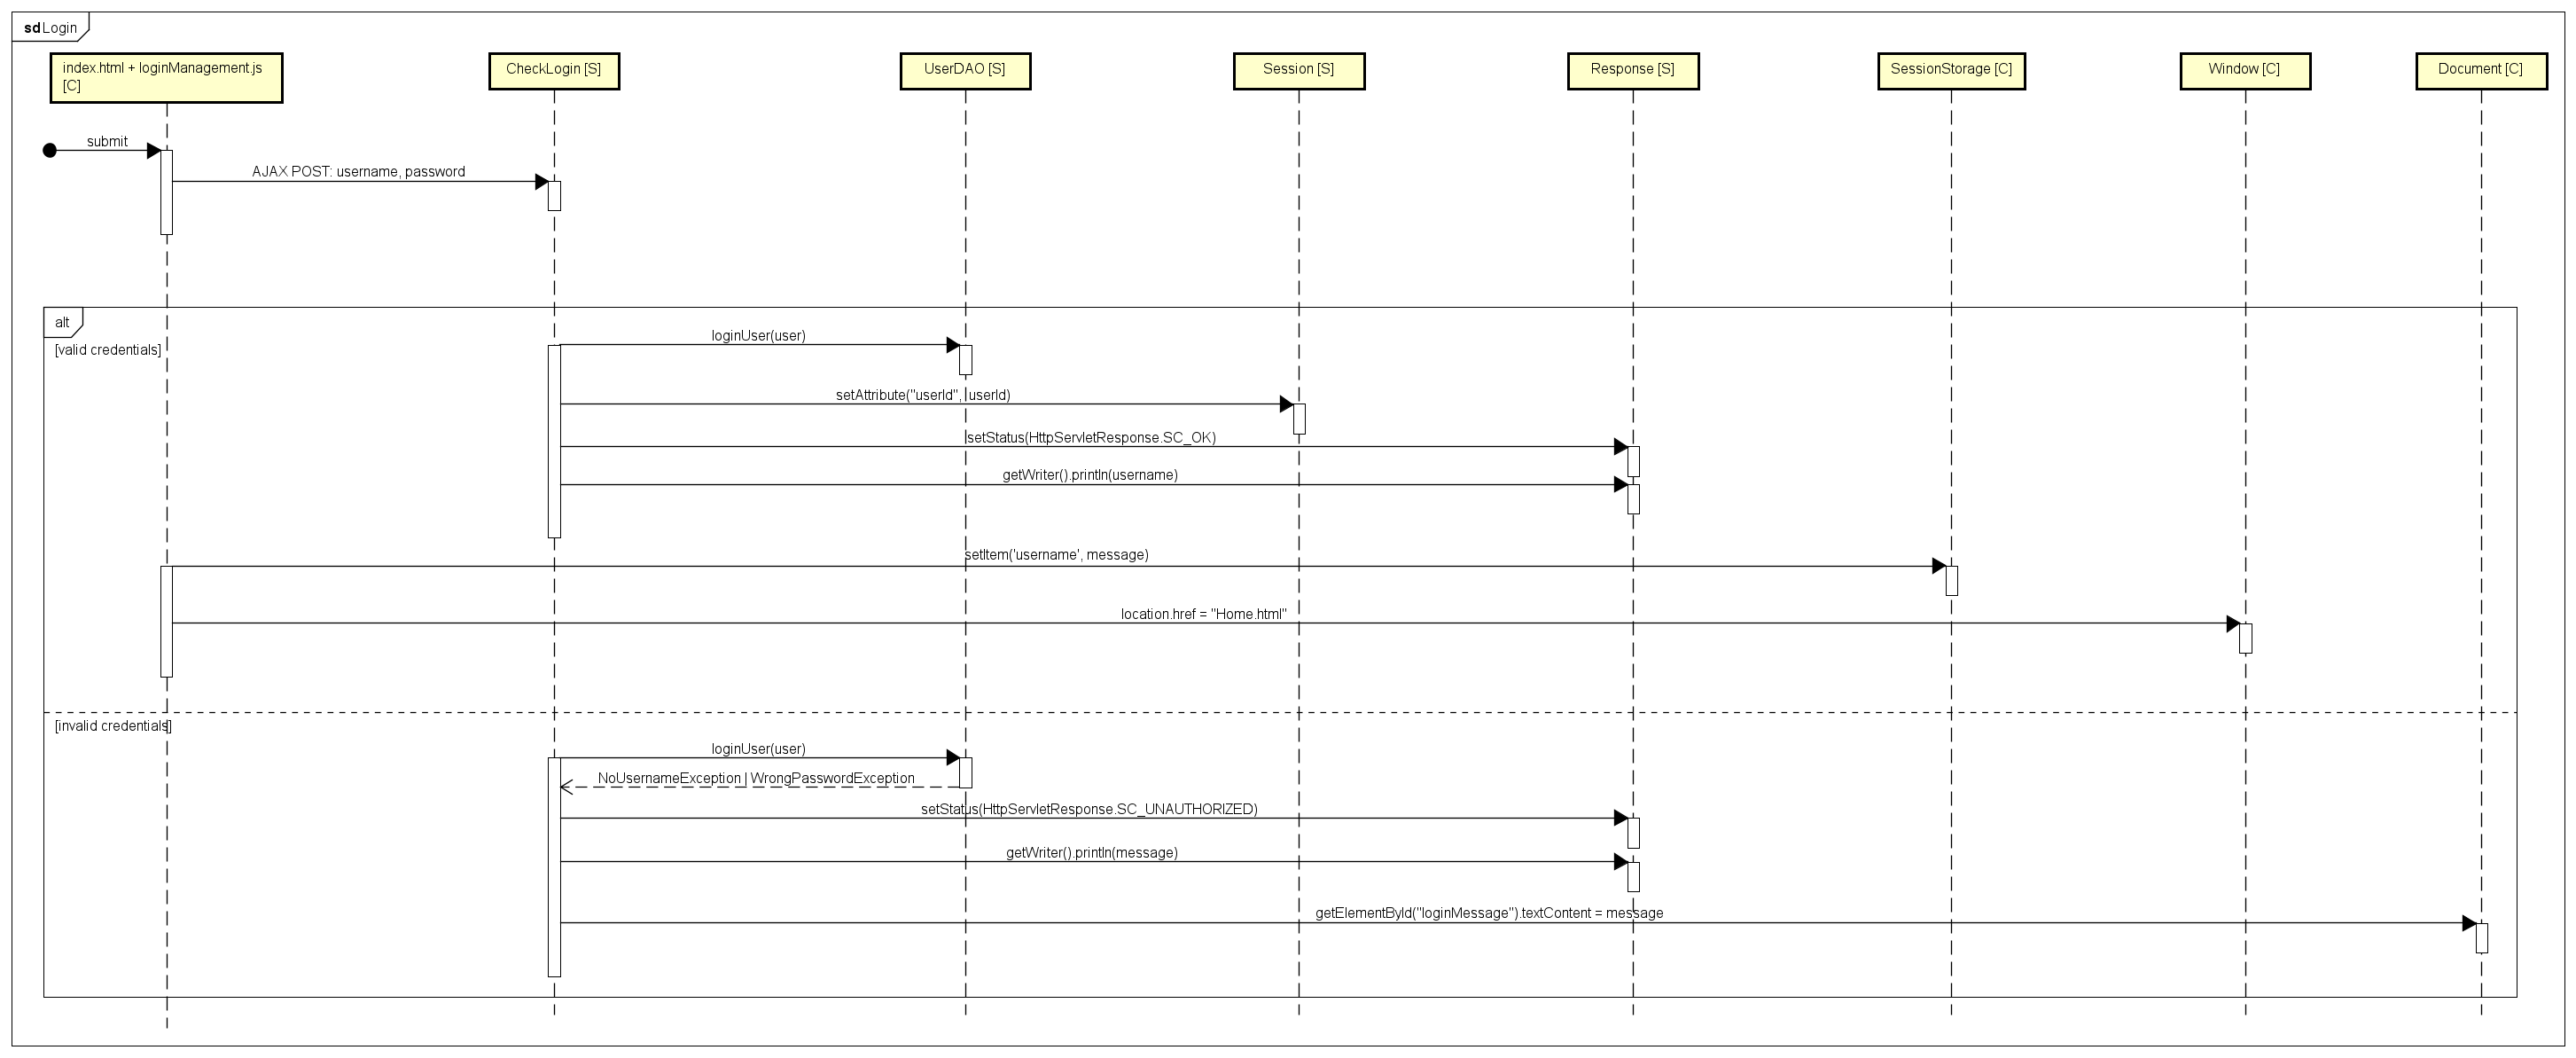
\includegraphics[width=1.0\textwidth]{JS/SequenceDiagram/Login.png}
    \caption{Login sequence.}
\end{figure}

\begin{figure}[H]
    \centering
     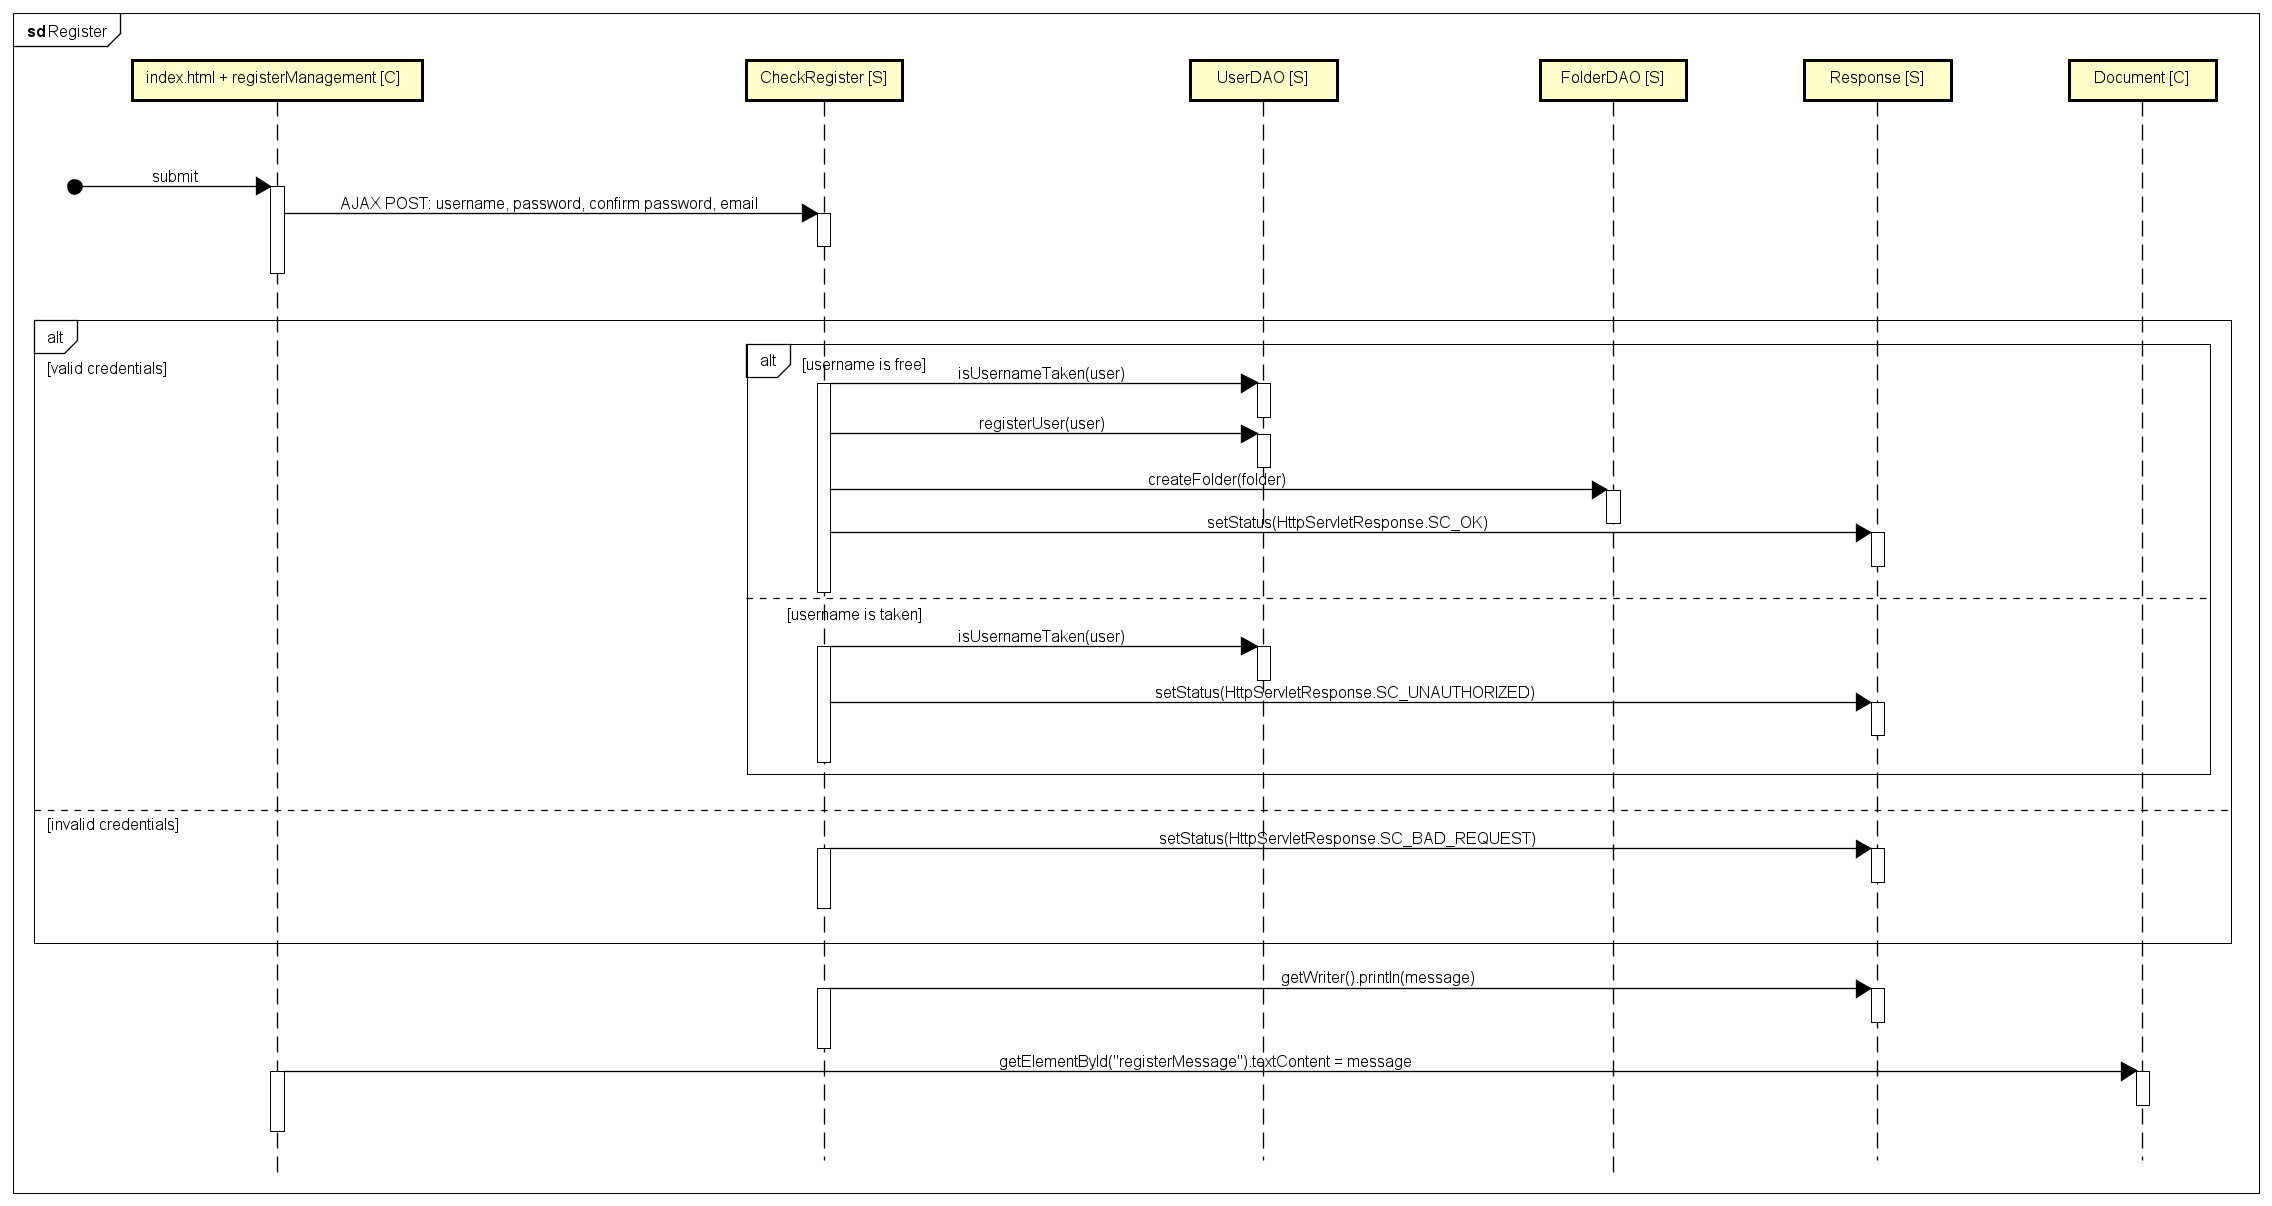
\includegraphics[width=1.0\textwidth]{JS/SequenceDiagram/Register.png}
    \caption{Register sequence.}
\end{figure}

\begin{figure}[H]
    \centering
     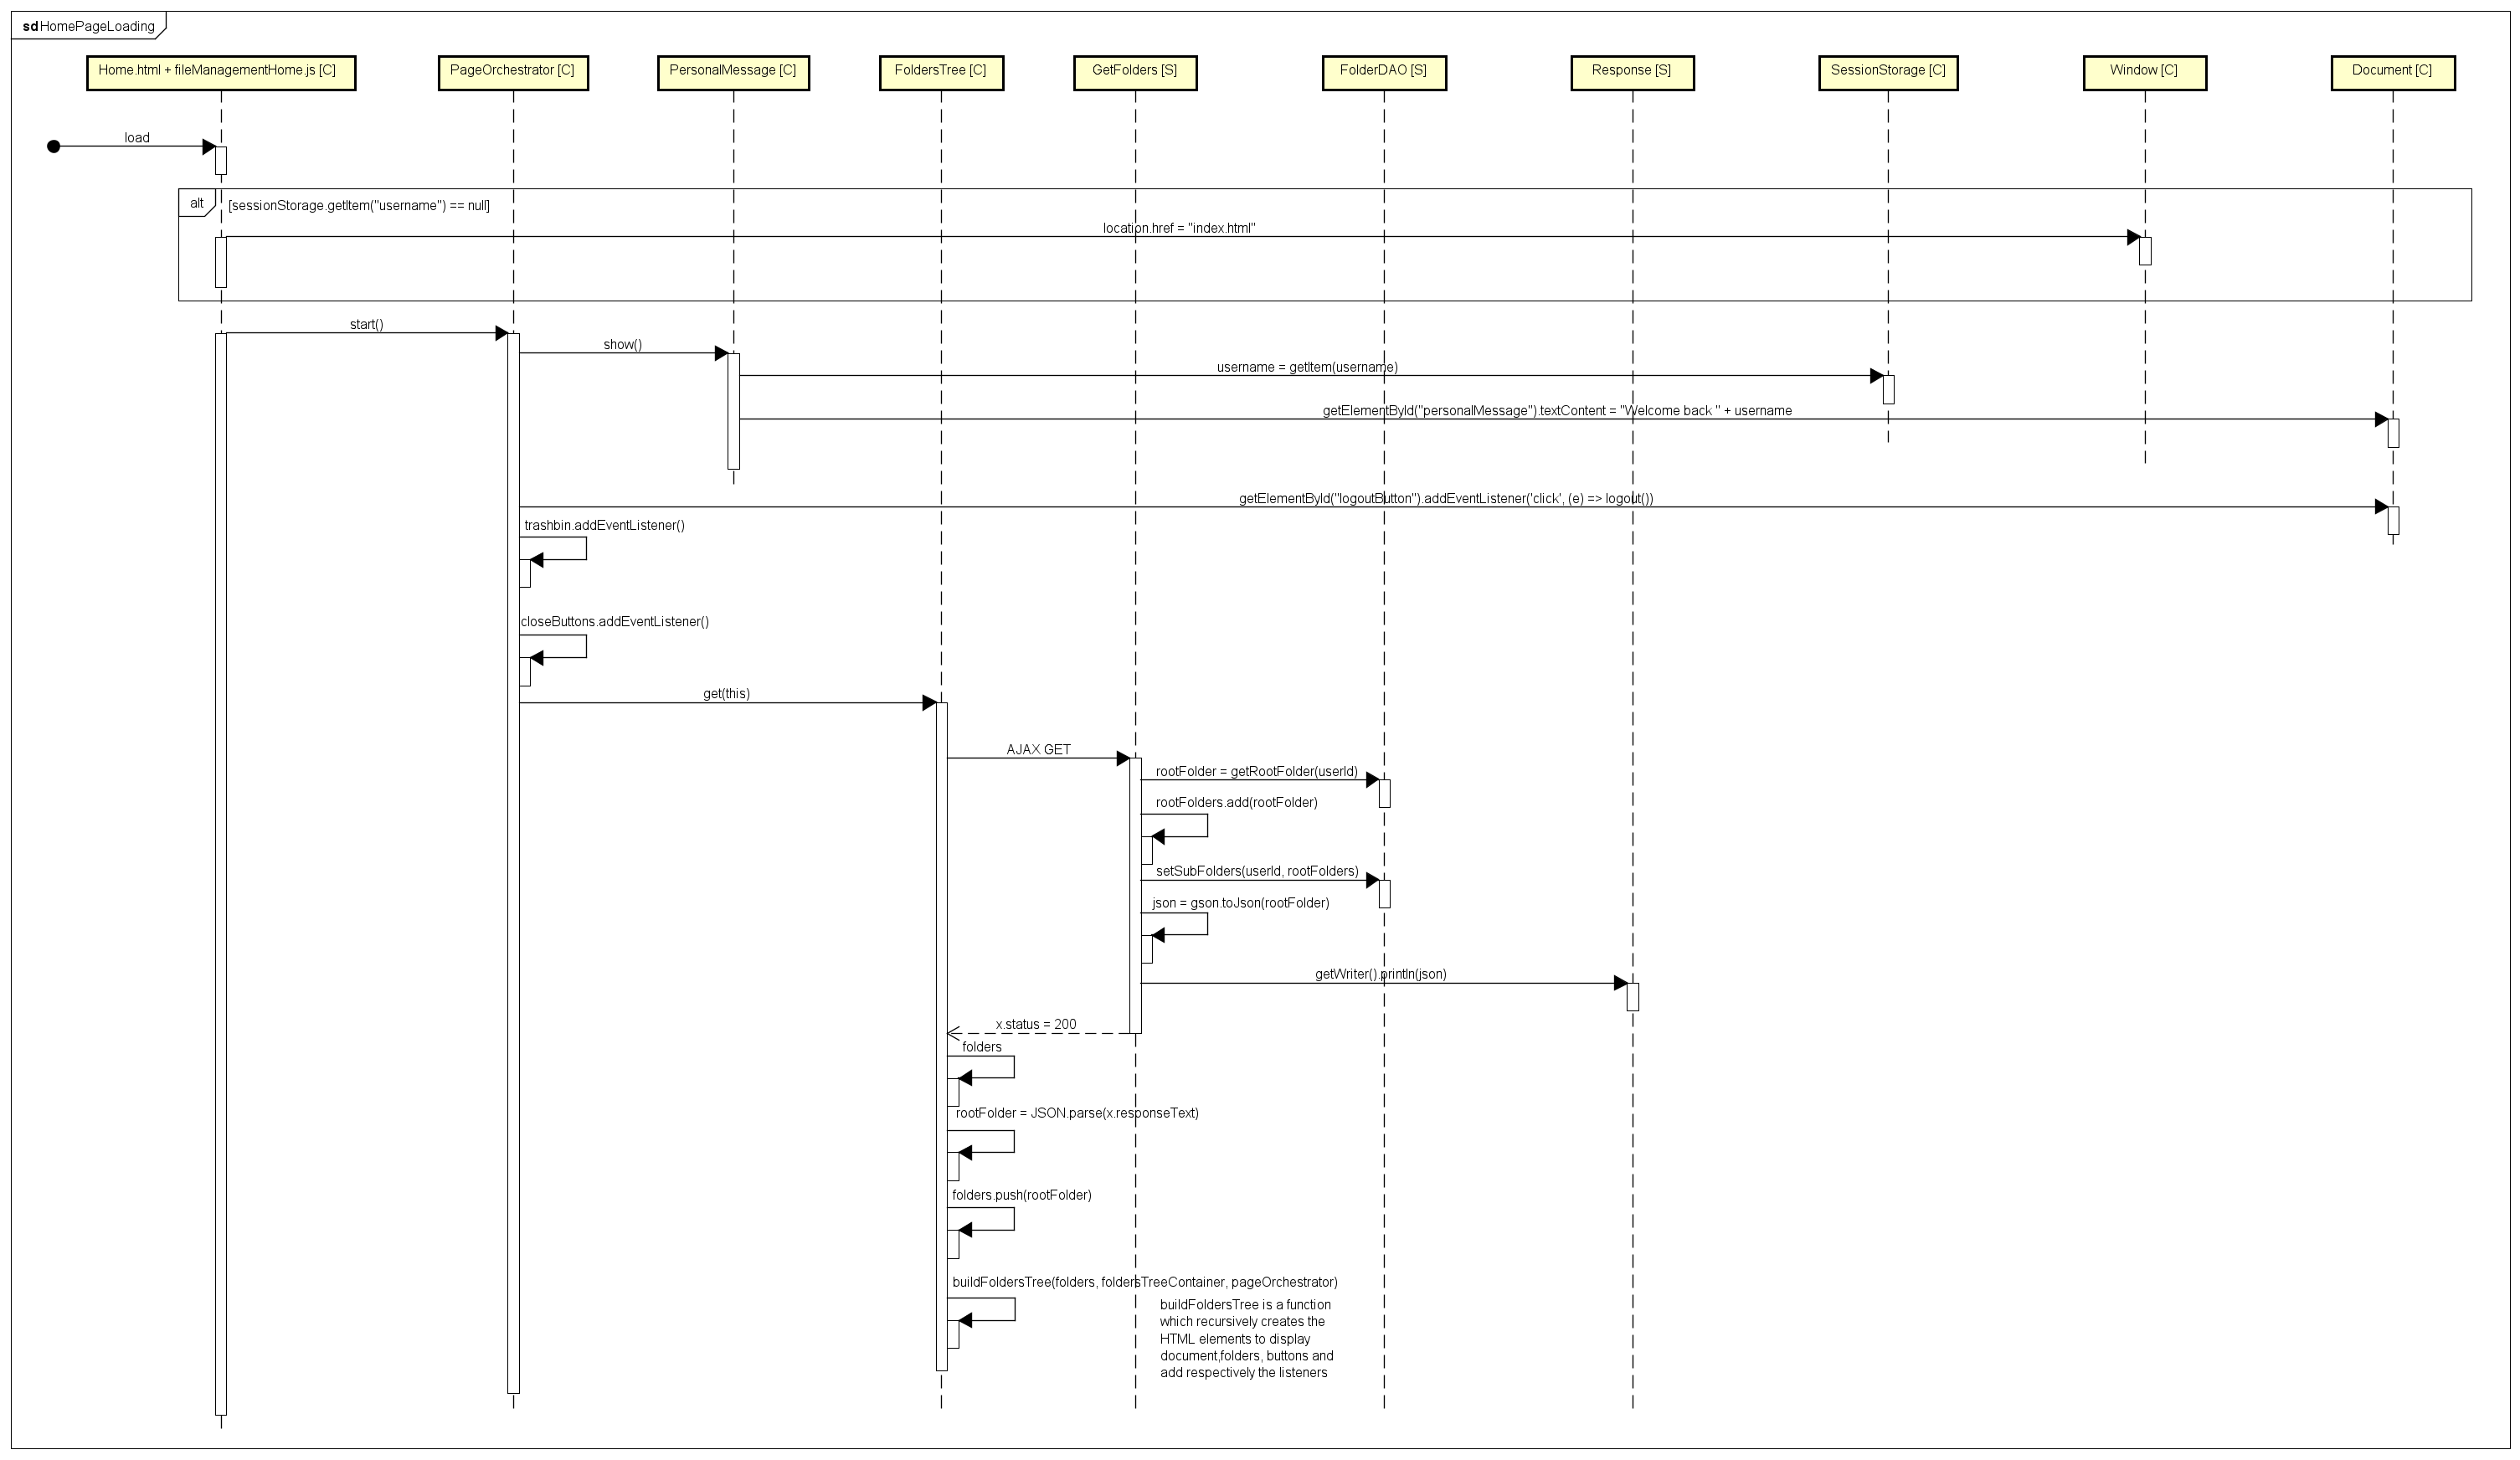
\includegraphics[width=1.0\textwidth]{JS/SequenceDiagram/HomePageLoading.png}
    \caption{Home page loading sequence.}
\end{figure}

\begin{figure}[H]
    \centering
     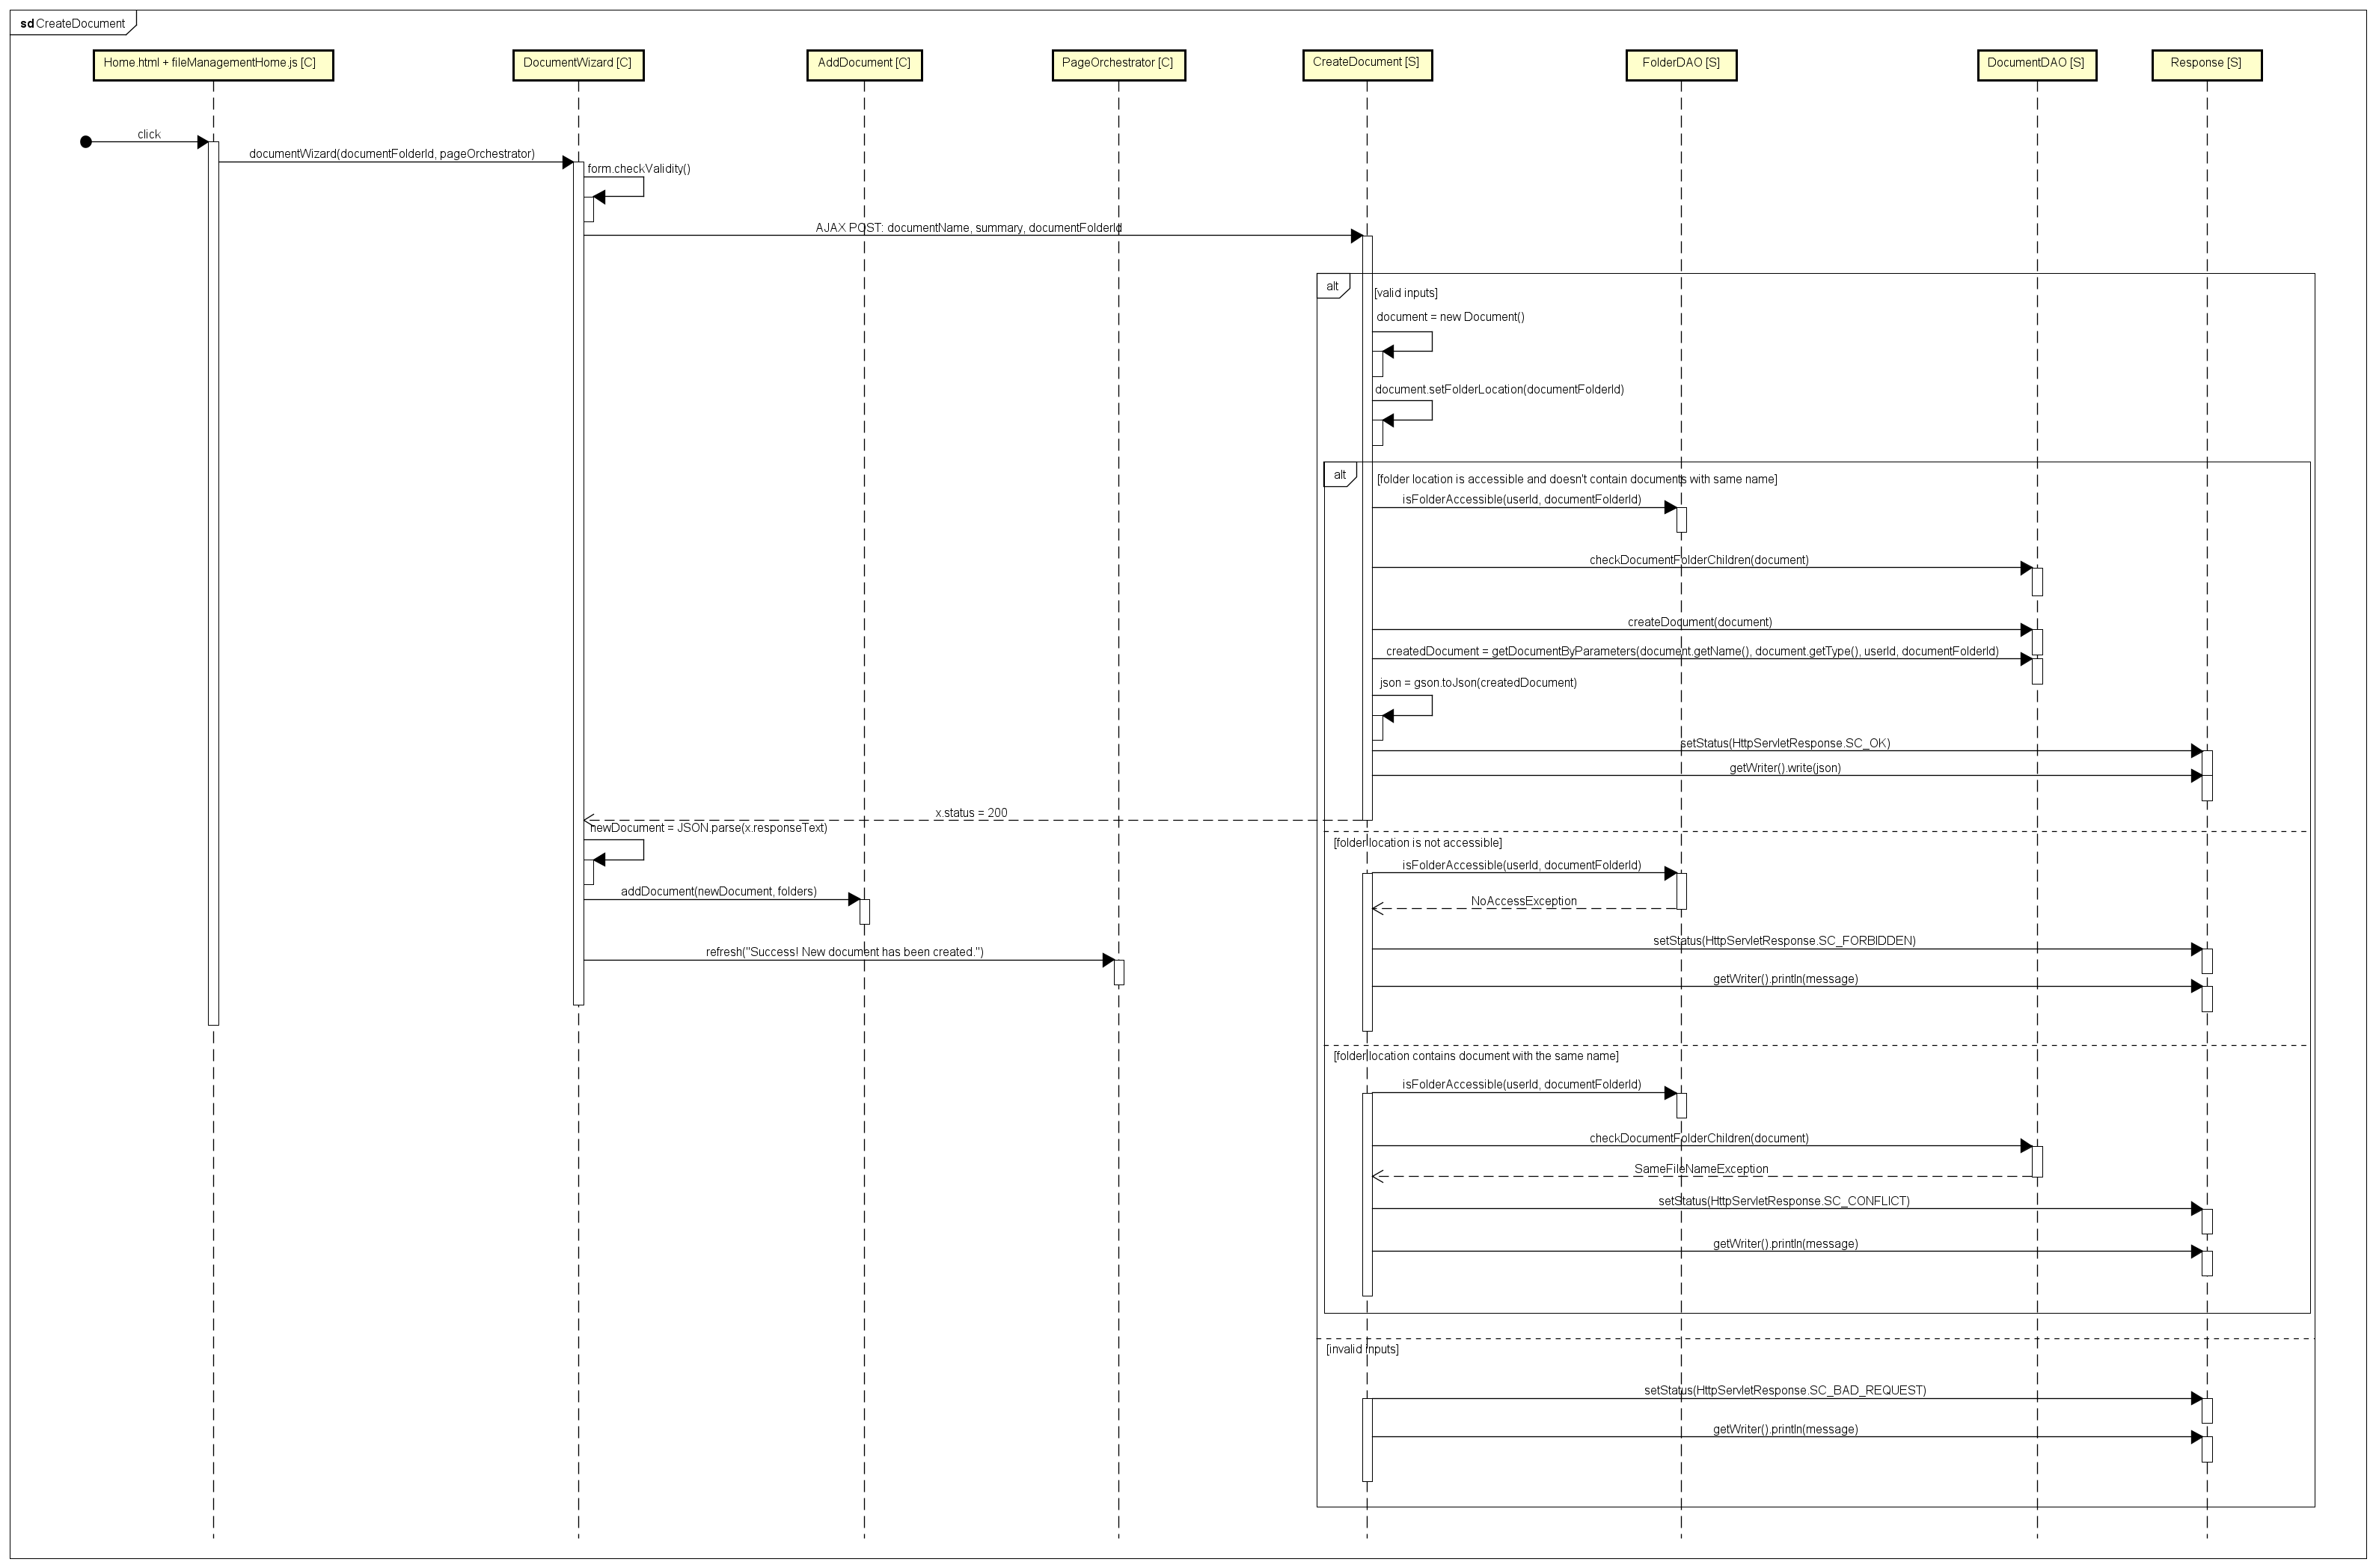
\includegraphics[width=1.0\textwidth]{JS/SequenceDiagram/CreateDocument.png}
    \caption{Creating a document sequence.}
\end{figure}
    
\begin{figure}[H]
    \centering
     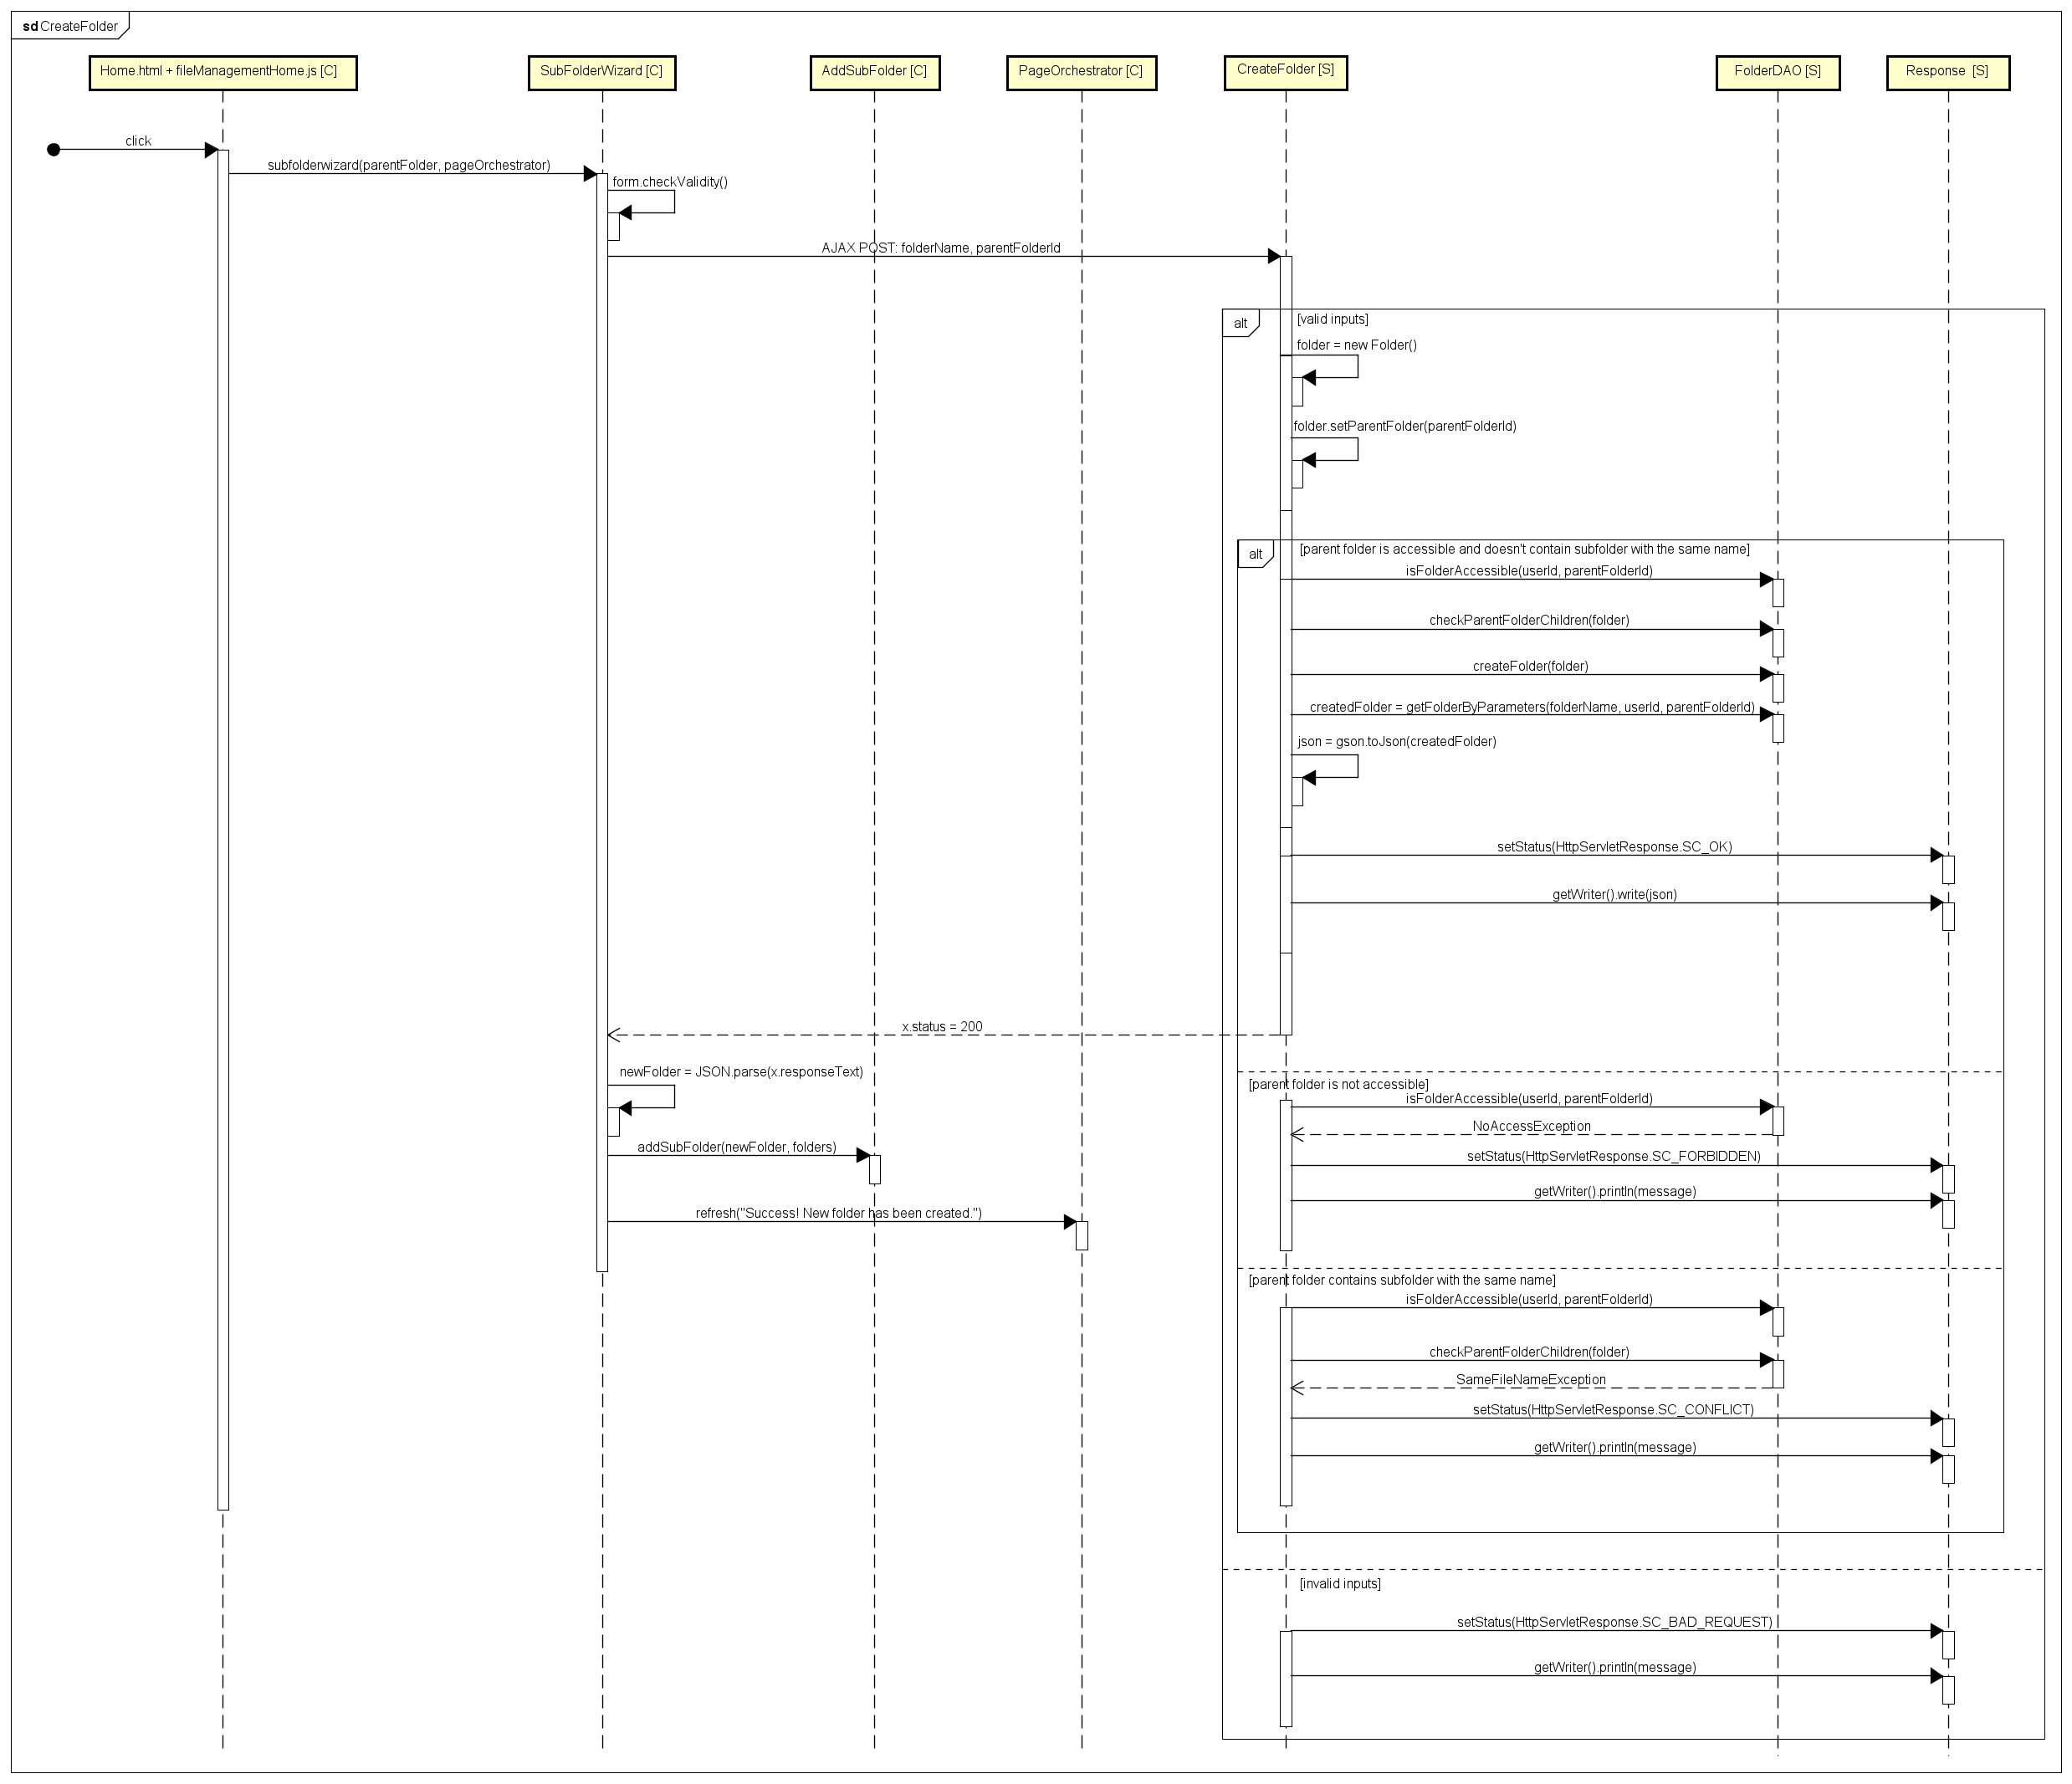
\includegraphics[width=1.0\textwidth]{JS/SequenceDiagram/CreateFolder.png}
    \caption{Creating a folder sequence.}
\end{figure}
        
\begin{figure}[H]
    \centering
     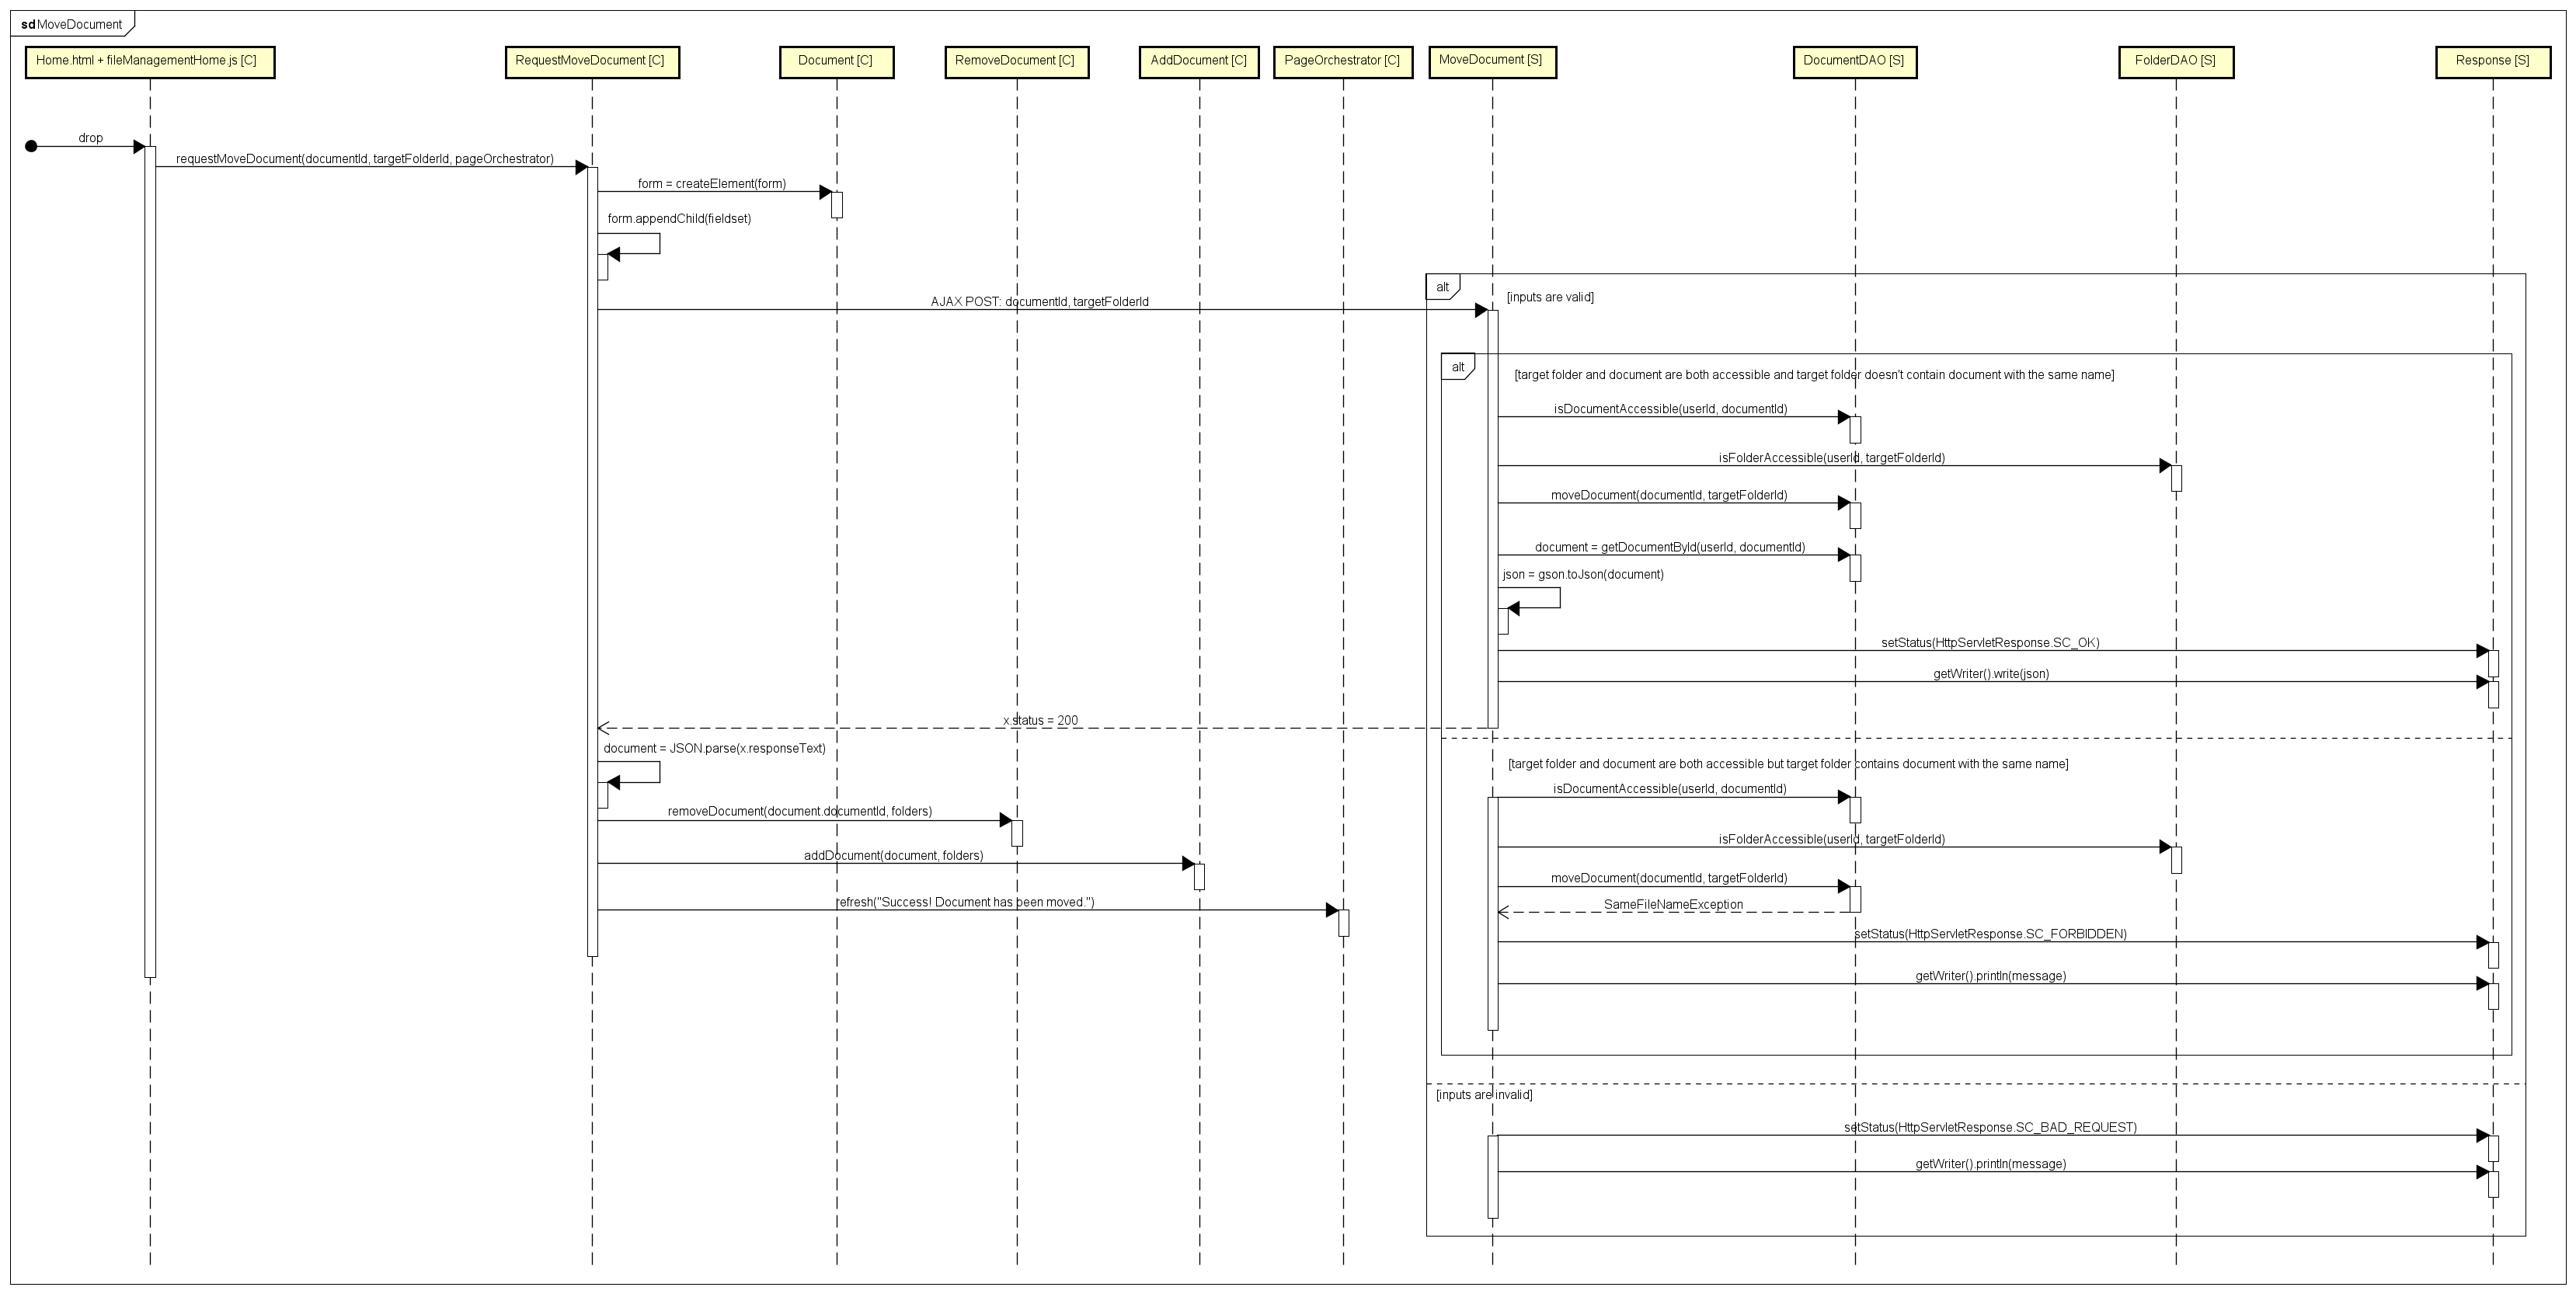
\includegraphics[width=1.0\textwidth]{JS/SequenceDiagram/MoveDocument.png}
    \caption{Moving a document sequence.}
\end{figure}
    
\begin{figure}[H]
    \centering
     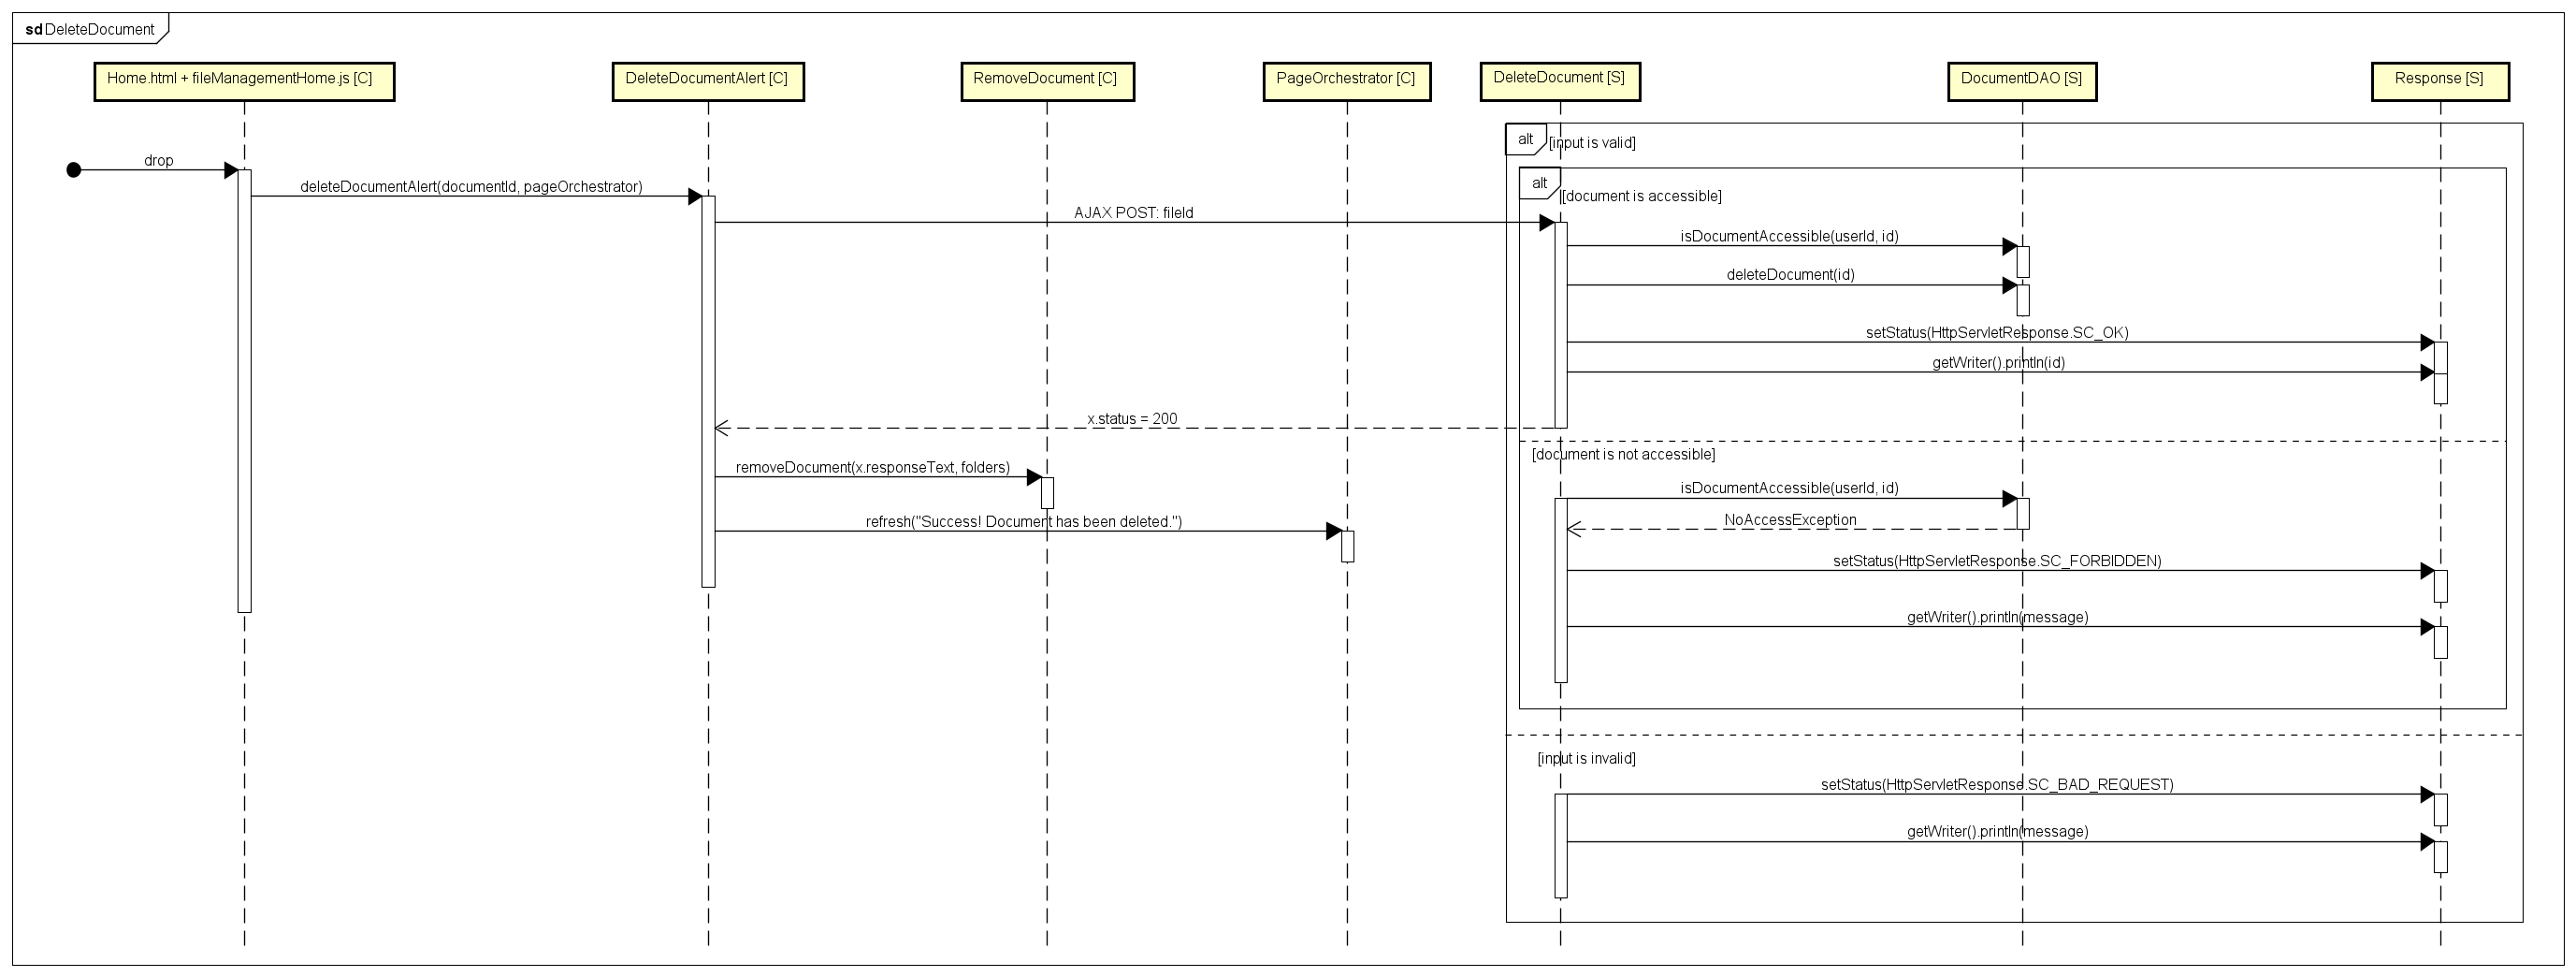
\includegraphics[width=1.0\textwidth]{JS/SequenceDiagram/DeleteDocument.png}
    \caption{Deleting a document sequence.}
\end{figure}    

\begin{figure}[H]
    \centering
     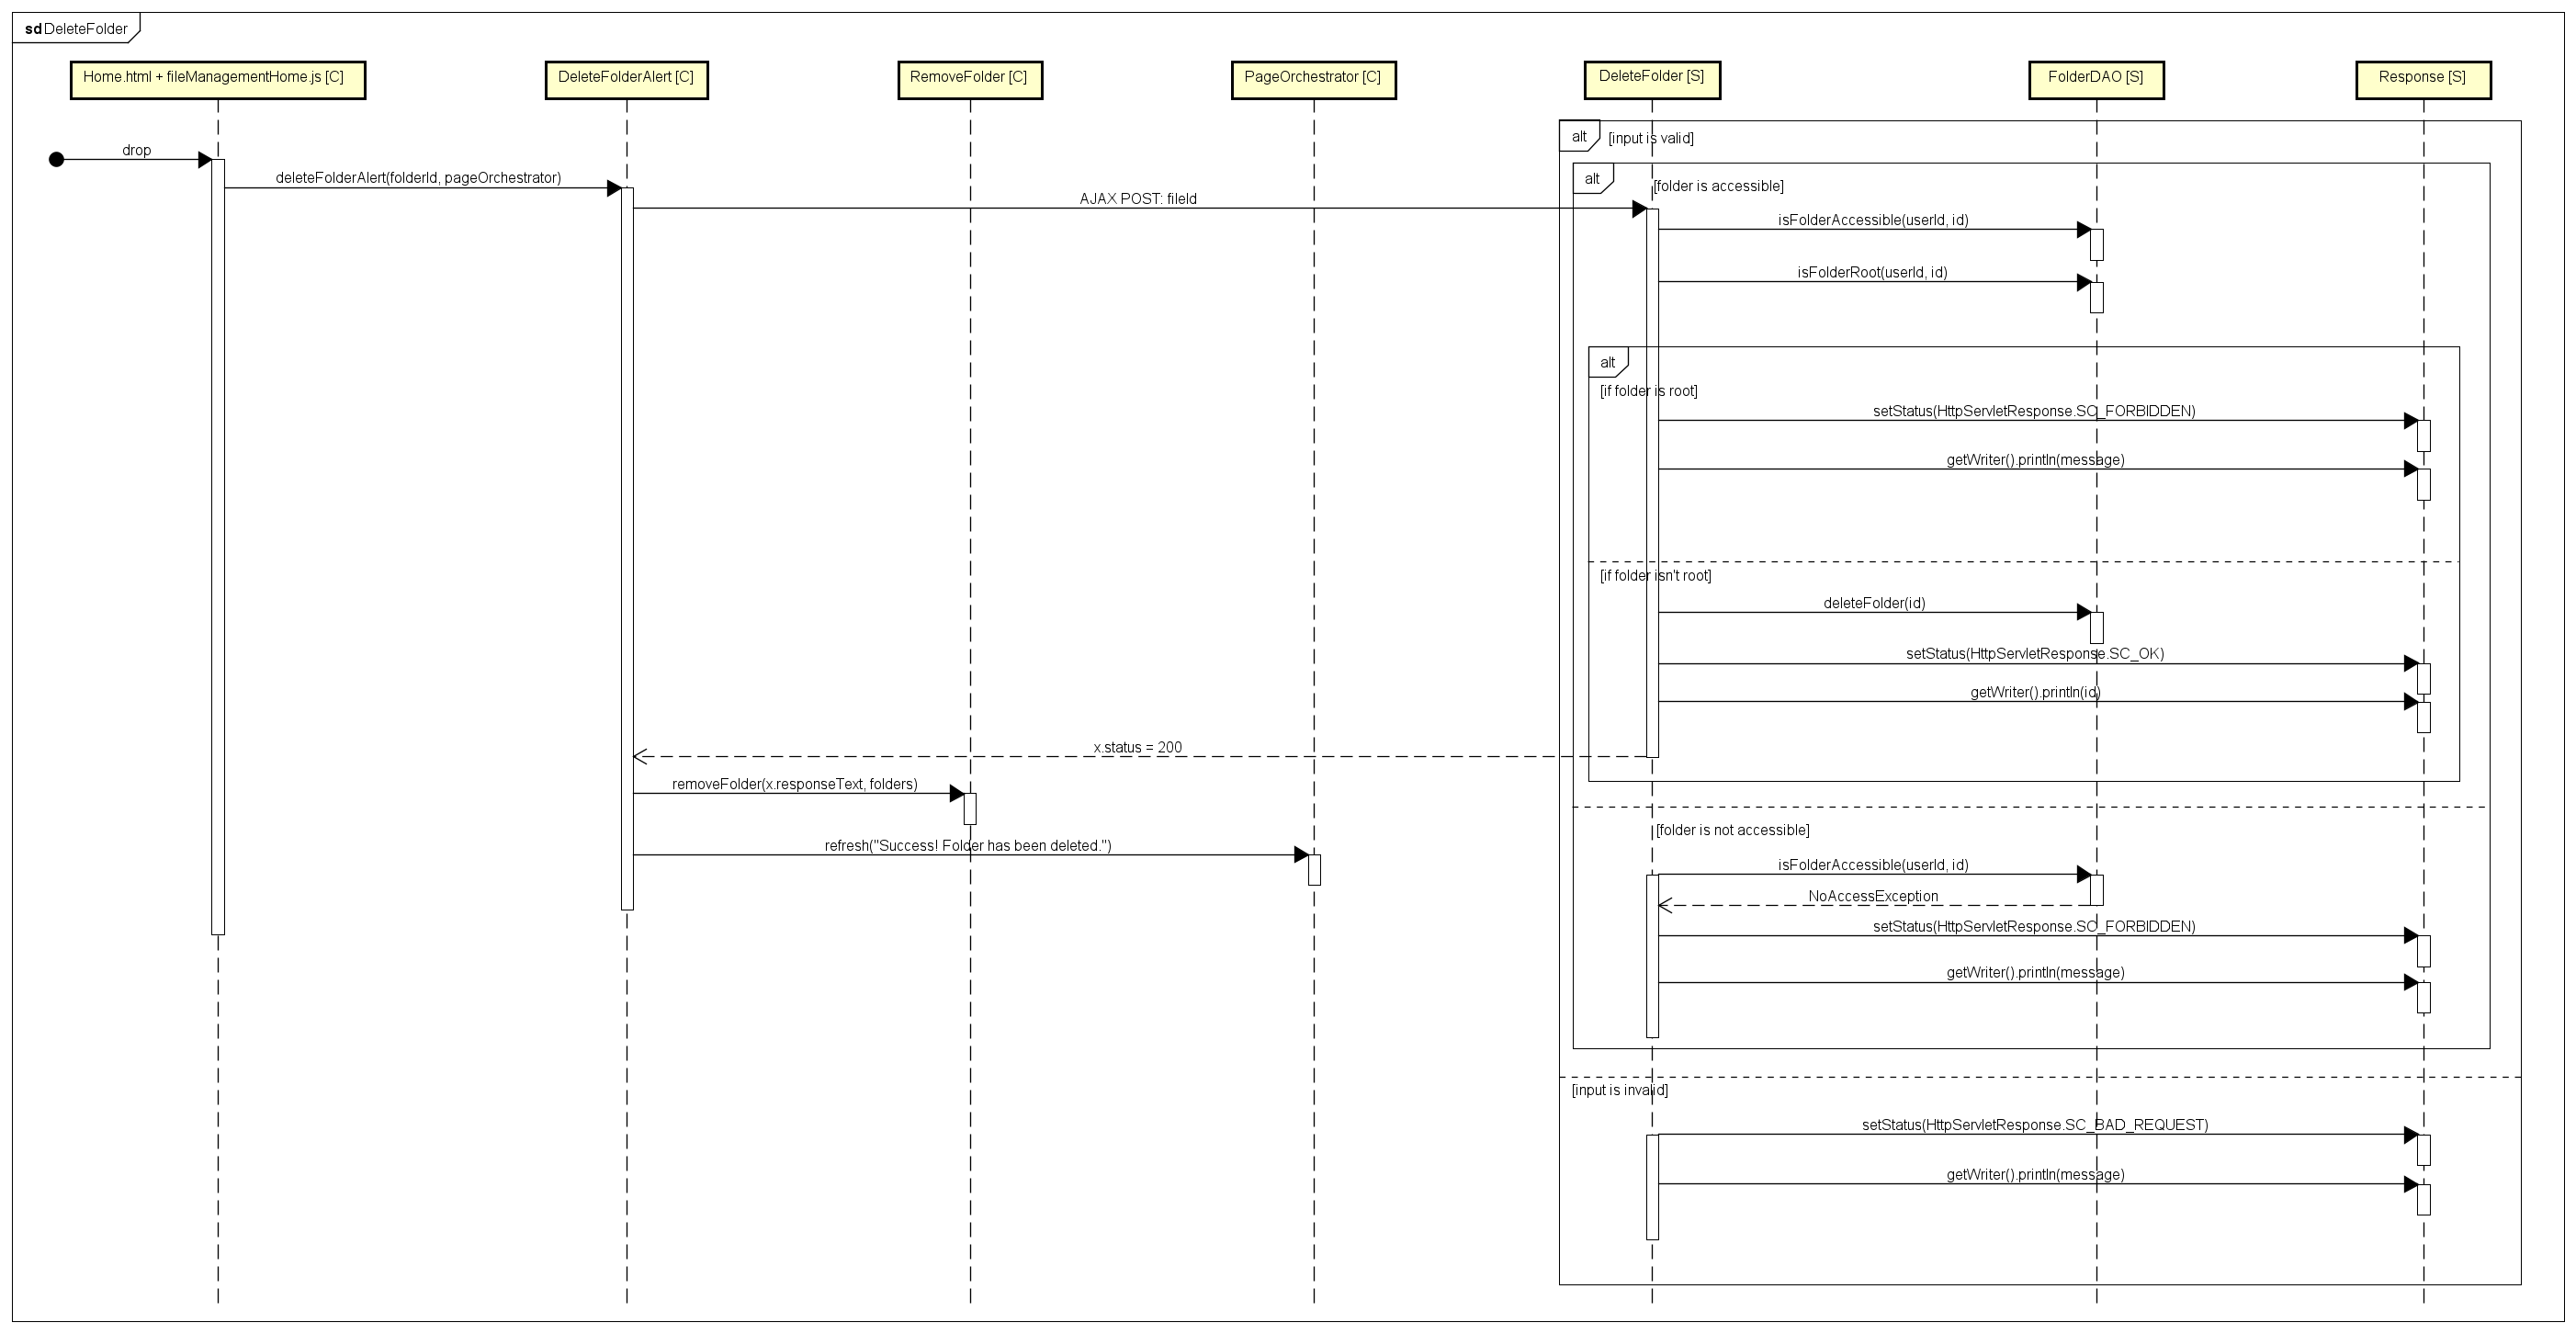
\includegraphics[width=1.0\textwidth]{JS/SequenceDiagram/DeleteFolder.png}
    \caption{Deleting a folder sequence.}
\end{figure}
    
\begin{figure}[H]
    \centering
     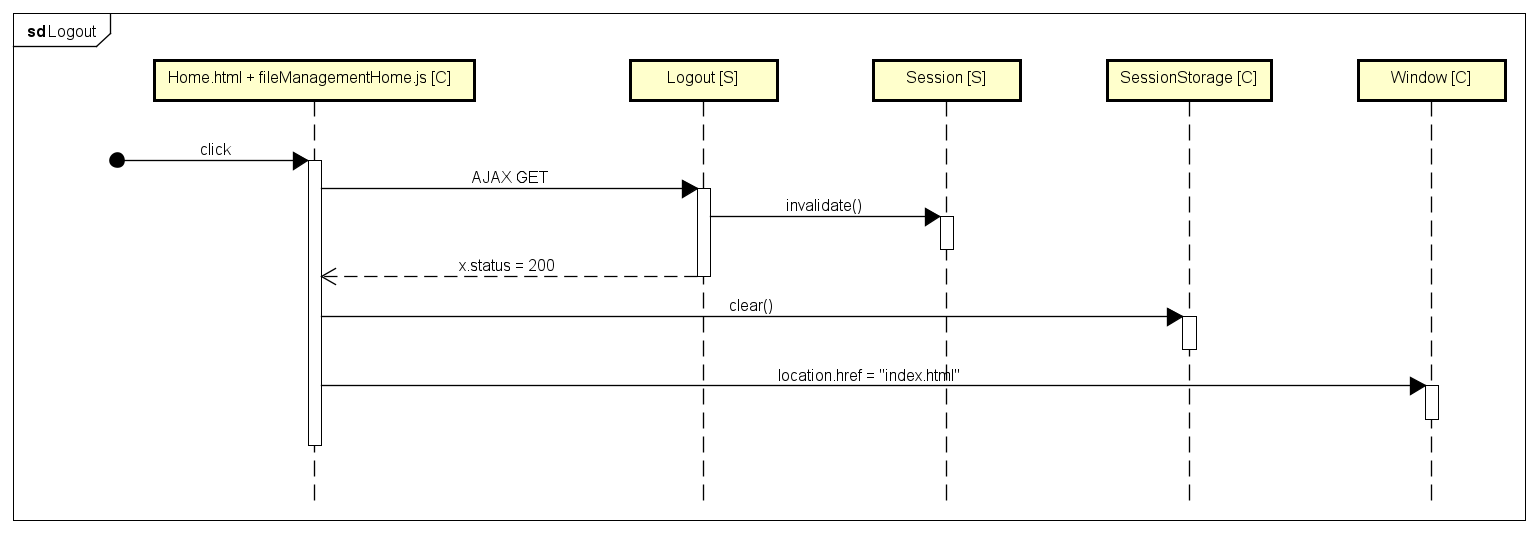
\includegraphics[width=1.0\textwidth]{JS/SequenceDiagram/Logout.png}
    \caption{Logout sequence.}
\end{figure}

\newpage
\section{Final considerations}
The application can be considered a success as it fully meets the project requirements of creating a file system website. The implementation leverages multiple technologies, including HTML, CSS, Java, JavaScript, Thymeleaf, and SQL, all of which were seamlessly integrated to develop a complete and functional application.\\
One of the greatest challenges I encountered during this project was understanding and utilizing JavaScript, a language I had never used before. Fortunately, the resources provided by the instructors, particularly on writing JavaScript and making AJAX requests, were invaluable in overcoming this hurdle.
My workflow began with designing the database, which I iterated on two to three times before finalizing the current structure. I am particularly proud of the database design, as I believe it is the most efficient and robust aspect of the project.\\
The application also has potential for future improvements, such as introducing an admin role with the ability to view all folders and documents across users or implementing the functionality to move folders, which was outside the scope of this project.\\
This project has been instrumental in solidifying my skills in Java and in designing complex web applications. The experience of integrating diverse technologies and managing data within an SQL environment proved to be both challenging and rewarding. Overcoming these challenges significantly enhanced my problem-solving abilities. The final product is a functional, scalable solution with ample room for further enhancements and features.
        
\end{document}
